\chapter{Implementation}\label{ch:implementation}

The previous sections explained \textit{what} the application should do, which goals should be achieved and which requirements we surely want the application to meet. In this section, more details are provided about \textit{how} all this is translated to an implementation.

\section{Web Application}
Before we started with the actual implementation, we had to decide how to achieve \ref{goal:device-os-independent}, i.e. how will we make sure the application is device- and OS-independent? (Requirement section \ref{sec:other-requirements}) A first technique could have been to make use of the Java Virtual Machine. This approach would work but we want to make it possible to let multiple people work on the same visualization (\ref{fr:work-simultaneously}), eventually at the same time. Therefore, it is more convenient to have a browser-based application, i.e. Web Application.\\

Nowadays, a lot of browsers exist, each with their own characteristics and differences. Because the goal of this thesis was to have a functional prototype, it is not required that the application works perfectly on \textit{all} possible browsers. However, we wanted to make sure that the tool works without any issues in one of the most popular browsers, being Google Chrome.\\

\textcolor{blue}{
Another possibility would have been to use cross-platform tools like PhoneGap\footnote{\url{https://phonegap.com/}} and Cordova\footnote{\url{https://cordova.apache.org/}}. The benefit of those tools is that, if a real application is preferable to a browser-based application, it is still possible to wrap the browser app into a real app. Hence, from then on the application can be installed on the device itself. A drawback of this is that the app cannot be used if the device has not enough disk space. Further, the app is possibly not up-to-date at any time. This can become an issue when the app would be collaborative and multiple users with different versions of the app want to work with it. Therefore, we concluded that a browser-based solution is better for our goal than the Java Virtual Machine and cross-platform tools.
}

% --------------------
% --- TECHNOLOGIES ---
% --------------------
\section{Used Technologies}\label{sec:technologies}
A lot of technologies exist to create Web applications and visualizations. A number of technologies assist in the developing process of such an application. In the following subsections we present the selected technologies, as well as why we chose for this particular technology and not for the alternatives.

\subsection{ReactJS}\label{sec:reactjs}
ReactJS\footnote{\url{https://reactjs.org/index.html}} is an open source library to create user interfaces. One of its main goals is to provide the best possible rendering performances\footnote{\url{https://medium.com/@thinkwik/why-reactjs-is-gaining-so-much-popularity-these-days-c3aa686ec0b3}}. Performance is good because ReactJS allows developers to break down the user interface into different components. Each component has its own \textit{state}, which contains information about the content of the component. This state can be updated while the application is running and if such an update is made, only this component is re-rendered instead of re-rendering the complete UI\footnote{\url{https://facebook.github.io/react/docs/why-react.html}}. Hence, this provides a huge benefit for the performance. Next to that, it is also not very hard to learn to code in React comparing to other frameworks (e.g. AngularJS). If the developer knows HTML and JavaScript, he will be able to code in ReactJS quickly.\\

Because of these benefits, ReactJS is the framework in which the GuideaMaps application is implemented. Each node and each link is considered as a separate and unique React Component. The most important reason for implementing the nodes like this is performance: if the state of the node is updated, only this node is re-rendered and not the complete UI.\\

Alternatives for ReactJS are for example AngularJS and VueJS\footnote{https://medium.com/@TechMagic/reactjs-vs-angular5-vs-vue-js-what-to-choose-in-2018-b91e028fa91d}. ReactJS is by far the most used of these three. Further, it is said to be easier to learn because you only have one structure (``Component''), while in AngularJS this is not the case. Also, VueJS lacks resources and is not used a lot in practice, which makes it more difficult to discuss problems with other developers. Maybe the most important benefit of ReactJS is its performance; React is really fast and our tool should have fast rendering times as well. Hence, because the alternatives seem to have some important drawbacks, we chose for ReactJS as the framework for creating the application. 

\subsection{d3}\label{sec:d3}
Another helpful tool is d3. With d3-hierarchy\footnote{\url{https://github.com/d3/d3-hierarchy}}, it is possible to transform JSON-data into hierarchical data. Having this kind of data makes it much easier to create a tree- or cluster-structure. In the case of GuideaMaps, a clustered visualization is very useful. The \textit{main}-node (a.k.a. the root node) is then positioned at the center, such that its child nodes can be placed around it. Hence, the further a node is away from the center, the lower it is in the hierarchy. Also, the visualization will not be messed up by positioning the nodes in this way, because every node has exactly one parent. This means there will not be a spaghetti of links where you cannot see from which node the link comes and to which node it is pointing.\\

Further, d3 makes it easier to create a zoomable layout. The tool is able to update the positions of the nodes each time the zooming level is changed. Hence, as a developer, you do not have to take care of the updated positions if you make use of d3. By using this technique, the functional requirements about zooming (\ref{fr:zoom} and \ref{fr:zoom-to-fit}) are easily achieved.\\

The alternatives for d3 most of the time come with a problem d3 does not have. For example ChartJS and ChartistJS are limited in the number of features: you can create nice charts with it, but d3 provides more visualizations than only charts. Further, some of the alternatives are commercial (Highcharts, Webix). d3 is open-source and provides functionality to zoom, to create a cluster of nodes based on JSON-data describing these nodes, etc. Because of the wide range of possibilities with d3, the fact that it is widely used and supported by all modern browsers and that it is able to act together with ReactJS, we believe that d3 was a better choice than its alternatives. 

\subsection{Tailwind CSS}\label{sec:tailwind}
Nowadays, the ``look and feel'' of an application is very important. Everything should look pretty and, as already mentioned in section \ref{sec:usability-requirements}, the actions should be straightforward and visible. Implementing a nice style can require a lot of code. The code for these styles can become a big part of the implementation. Hence, a good framework is necessary to reduce the lines of style code to a reasonable number and to help to improve the readability of the code.\\

Tailwind CSS\footnote{\url{https://tailwindcss.com/}} is a framework that assists developers to style their application. The difference with more famous frameworks, like Bootstrap, is that Tailwind CSS has no default theme. If you want to use a Bootstrap-feature, this eventually comes along with other features you do not always want and it can be quite hard to undo the part you do not want. Furthermore, you have to write additional lines of style code to undo the unwanted parts. With tailwind on the other hand, you can grab only the features you want, without side-effects. \autoref{fig:examplecode-tailwindcss} shows an example with two small listings. The first uses inline style while the second makes use of tailwind CSS.

\begin{figure}[H]
	\begin{minipage}[b]{0.5\textwidth}
 		\centering
  		\begin{minted}[linenos, escapeinside=||]{html}
<div
  style={{
    |\textcolor{red}{position:}| absolute|,|
    |\textcolor{red}{border:}| 1px solid black|,|
    |\textcolor{red}{borderRadius:}| O.25rem|,|
    |\textcolor{red}{padding:}| 0.5rem|,|
  |\textcolor{red}{\}\}}|
/>
		\end{minted}
		\label{lst:no-tailwind}
		\captionof{lstlisting}{Normal CSS, no tailwind.}
	\end{minipage}
 	\begin{minipage}[b]{0.5\textwidth}
  		\centering
		\begin{minted}[breaklines, escapeinside=||]{html}
<div
  className={
    |'|absolute border border-solid border-black rounded p-2|'|
  |\textcolor{red}{\}}|
/>
		\end{minted}
		\label{lst:tailwind}
 	 	\captionof{lstlisting}{With tailwind CSS.}
 	\end{minipage}
	\caption{Difference when using tailwind CSS or not.}
	\label{fig:examplecode-tailwindcss}
\end{figure}

The figure illustrates the difference to implement four CSS property-value pairs in normal CSS and implementing the same four with tailwind. In the case of normal CSS, we need four lines of code to obtain the intended result. On the other hand, with tailwind CSS, we add some classes providing the same style. By using these classnames, the developer can see the properties faster than with normal CSS. Hence, in case of lots of lines of CSS code, tailwind can be faster to use compared to normal CSS.\\

Bootstrap can be very interesting to use in applications and websites that should run on devices with small screens (e.g. smartphones). But we decided not to tailor our application for such devices (section \ref{sec:other-requirements}). Given the example and the fact that Tailwind CSS does not have a default theme, we prefer Tailwind over Bootstrap. Keep in mind that it is certainly possible to create the same application with Bootstrap, but with Tailwind CSS, the code will be easier to understand.\\





% ---------------------
% ----- STRUCTURE -----
% ---------------------
\section{Main Code Structure}\label{sec:structure}
With the technologies mentioned in the previous section, the most important pillars the application relies on are discussed. In this section, we will explain the main structure of the code, such that it is clear how all elements work together. Figure \ref{fig:overall-structure} shows a visualization of the structure of the code.
\begin{figure}[H]
	\centering
	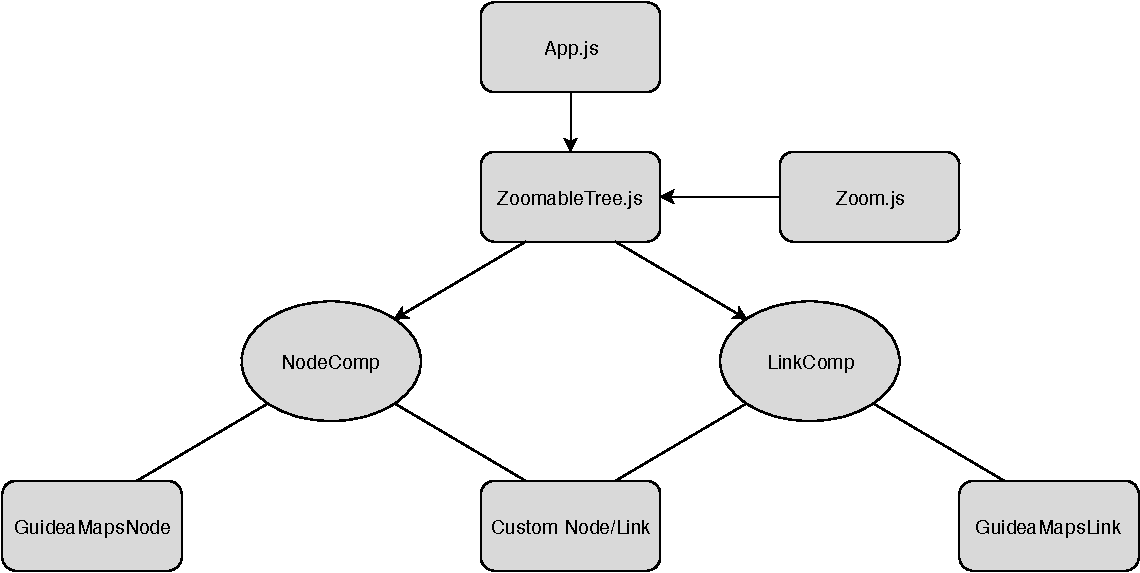
\includegraphics[width=\linewidth]{thesis-architecture.pdf}
	\caption{Structure of the application.}
	\label{fig:overall-structure}
\end{figure}

The application is developed in such a way that it can be used as a library for other purposes than GuideaMaps. In this way, \ref{goal:generic} to have a generic solution will be achieved. The general, always-returning part of the code can be found in App.js, ZoomableTree.js and Zoom.js, where the layout of the nodes is defined as well as the implementation to allow the user to zoom the visualization in and out. To realize the library, the layer of the NodeComp and LinkComp is very important. For GuideaMaps (shorthand GM), an implementation for NodeComp and LinkComp, being GMNode and GMLink is provided. Each implementation describes how every node and every link should look like in the visualization. When a particular user would like to have a different representation for the nodes or the links or both, new components (e.g. MyCustomNode and MyCustomLink) should be implemented. In the rest of the code, only one line should be adapted: in App.js, ZoomableTree is called with a certain number of props. Two of these props are NodeComp and LinkComp, which are set to GMNode and GMLink, respectively, by default. Hence, the only action that is required to \textit{plug in} an other component is replacing GMNode and GMLink by this component (e.g. MyCustomNode and/or MyCustomLink). Hence, the visualization can be customized to the needs of the user and \ref{fr:customization} is achieved. \autoref{fig:examplecode-library} shows the part of the code in App.js that should be adapted as explained. Note that the shown props are not the only props that are passed to ZoomableTree. The others are omitted for readability.\\

The reason why we chose for this approach is that now the developer does not have to change anything of the default implementation. He only has to create his own components and plug them in as props for ZoomableTree and leave the rest of the implementation as it is.\\

\begin{figure}[H]
	\begin{minipage}{0.5\textwidth}
 		 \centering
		 \begin{minted}[linenos, escapeinside=||]{html}
<ZoomableTree
    |\textcolor{mygreen}{NodeComp}|=|\textcolor{red}{\{GMNode\}}|
    |\textcolor{mygreen}{LinkComp}|=|\textcolor{red}{\{GMLink\}}|
/>
		\end{minted}
		\label{lst:default-components}
		\captionof{lstlisting}{Default components.}
	\end{minipage}
 	\begin{minipage}{0.5\textwidth}
  		\centering
  		\begin{minted}[escapeinside=||]{html}
<ZoomableTree
    |\textcolor{mygreen}{NodeComp}|=|\textcolor{red}{\{MyCustomNode\}}|
    |\textcolor{mygreen}{LinkComp}|=|\textcolor{red}{\{MyCustomLink\}}|
/>
		\end{minted}
		\label{lst:custom-components}
 	 	\captionof{lstlisting}{Custom components.}
 	\end{minipage}
	\caption{Two listings showing how to use the library.}
	\label{fig:examplecode-library}
 	%\captionof{figure}{Two listings showing the difference between the default and custom use of the library.}
\end{figure}

Next to custom components, a developer can also implement his own functions to handle changes in the visualization. For example, to add a new child node, GuideaMaps calls the function passed to the \textit{onAddNode}-prop (i.e. addGMChildNode). In a custom implementation, you can pass another function to this prop to make sure that other work is done. If you do not want to allow users to add child nodes, you do not have to remove this line but you just replace addGMChildNode by \textit{() -> null}, a function that does not do anything (because the library is created in a way to avoid changes in the default code structure). It is not wrong to keep addGMChildNode as parameter, but if the function would be called, this can lead to errors or wrong behaviour of the application. Therefore, we recommend to always pass \textit{() -> null} as argument to functions that should not be used. More details about the use of the library can be found in Chapter \ref{ch:usecase}, where a complete use case is elaborated.



% ------------------------------
% ----- GUIDEAMAPS DETAILS -----
% ------------------------------
\section{Default Implementation: GuideaMaps}
Now the overview of the structure of the application has been discussed, we will consider the GuideaMaps visualization and its implementation details in this section. An example visualization can be seen in \autoref{fig:guideamaps}.\\

The nodes represent a specific part of the data and the links illustrate the relation between the data (i.e. the nodes). Before we discuss the nodes into detail, we start with the \textit{navigation bar} above the visualization itself. This navigation bar is divided in three equal parts. In the center, the user can select via an option menu which map or template he wants to use. The name of the selected option is always visible. This functionality is available because the user should be able to switch between different tasks. In each task, the user can work with a different map or start a new map based on one of the existing templates, created by a map creator.\\

The right part of the navigation bar contains a single button. A click on this button makes sure the visualization is zoomed in such a way that all nodes fit in the window. This is one of the reasons why we mentioned in the requirements (section \ref{sec:other-requirements}) that the screen of the used device should not be too small. If the screen is too small, the nodes of a larger visualization will overlap each other because otherwise they would not fit all on the screen. When nodes overlap, a lot of information can be hidden and the visualization can become useless.

\begin{figure}[h]
	\centering
	\frame{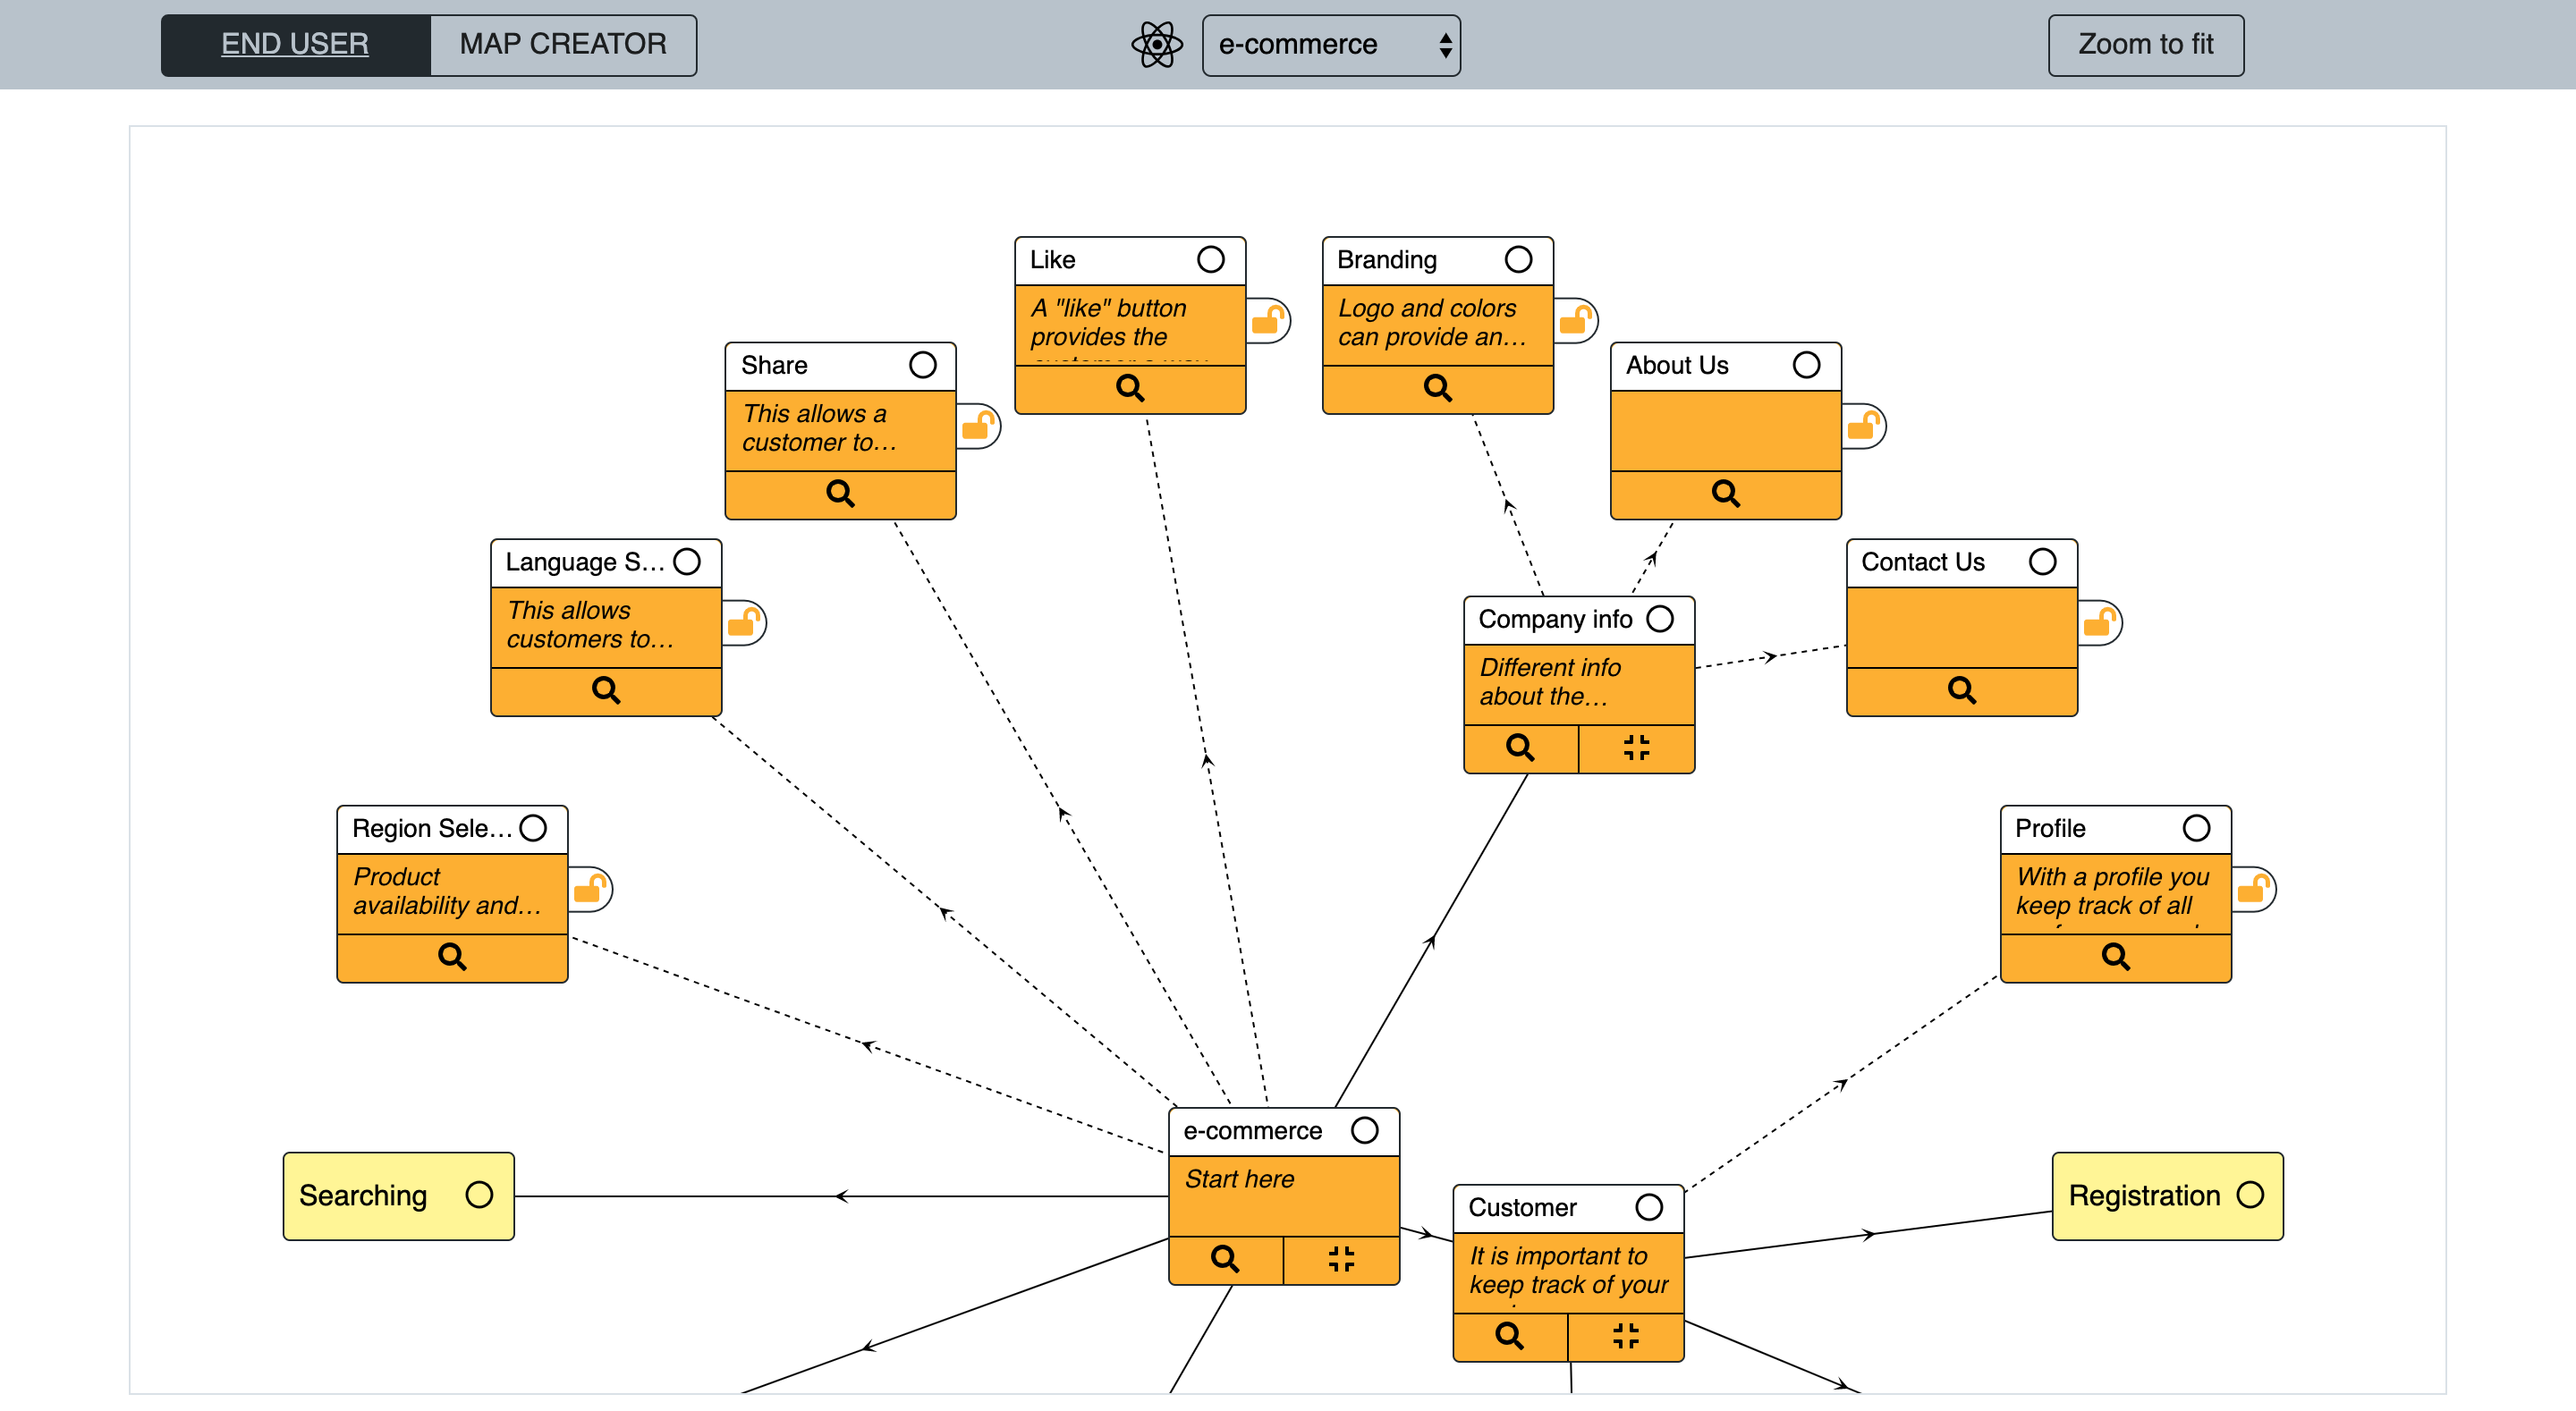
\includegraphics[width=\linewidth]{guideamaps.png}}
	\caption{GuideaMaps Layout.}
	\label{fig:guideamaps}
\end{figure}

The left part of the navigation bar is created to be able to switch between the user modes (i.e. end user or map creator). As required, a map creator has more rights and hence he can perform more actions than an end-user. In the following subsections, the differences between these modes are elaborated.





% ---------------------------
% ------ REGULAR NODES ------
% ---------------------------
\subsection{Regular Nodes}

\begin{figure}[H]
	\centering
	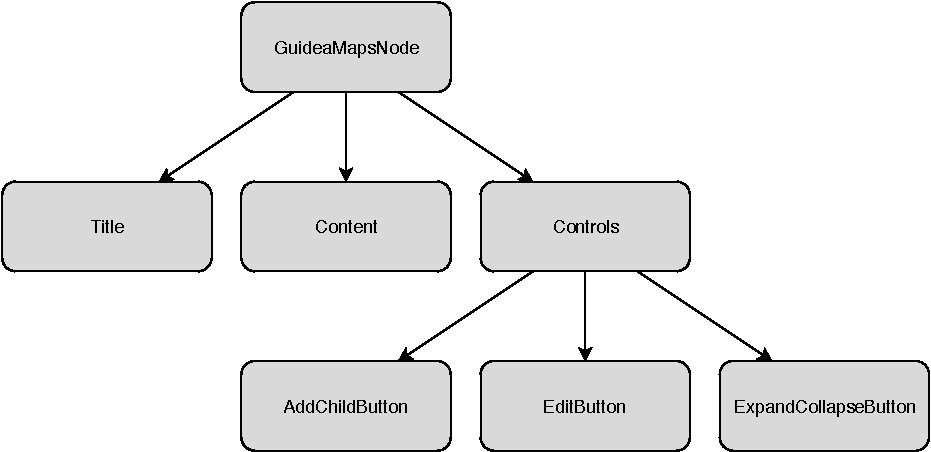
\includegraphics[width=\linewidth]{GMStructure.pdf}
	\caption{Structure of GuideaMapsNode.}
	\label{fig:gmnodestructure}
\end{figure}

As you can see in \autoref{fig:gmnodestructure}, the structure of a GuideaMapsNode node is quite simple. Each node consists of three html \textit{div}-elements: a title-div, a content-div and a controls-div explained below.

\addtocontents{toc}{\protect\setcounter{tocdepth}{2}} % hide the following subsections from the table of contents
\subsubsection{Title}
The title-div is positioned at the top of the node. It consists of the title text when this is given by the map creator. Otherwise, it shows \textit{Insert title} in italics to remind the user that he still has to set a title for this node. An end-user can set the title if no title exists yet, but he can never change it. The reason for this is because we distinguish two situations. In the first situation, the end-user adds a child node for a particular parent. This node has no title by default and then he should be able to insert a title. In the second situation, the user opens an existing node created by the map creator. In that case the end-user is not allowed to change the title of the node, because otherwise he would be able to change the meaning of the node. \\

Next to the title-text, the title-div contains an icon placed near the right border. This icon indicates to an end-user whether all information for the node, i.e. content, is provided or not. The icon that is shown also depends on whether the information in the child-nodes is given or not. We distinguish three possible situations:
\begin{enumerate}
	\item The node itself and all of its (non-optional) children are correctly filled in. In this case the icon will be a completely filled circle.
	\item The node itself and all of its (non-optional) children are still empty. In this case the icon will be an empty circle.
	\item In all other cases, the node itself or at least one of its child-nodes is filled. Then the icon will be a semi-filled circle.
\end{enumerate}
This icon can assist the end-user in determining whether all information requested by a template is given. For example, if he checks the root node and sees that the circle is completely filled, he knows that all mandatory information in every child-node is given. On the other hand, suppose only one node does not yet contain the required content, then the user starts from the root node and always follows the child-node with a semi-filled circle. In this way, he will find the incomplete node much faster than in the case he has to check all the nodes, one by one. Hence, the icon is an element that helps to improve the usability of the application.



\subsubsection{Content}\label{sec:content}
The content of each node is some text describing the information required for the node. As long as no content is provided by the end-user, the description provided by the map creator is shown in italics to instruct the end-user which content to provide.



\subsubsection{Controls}\label{sec:controls}
The last part of a node is the controls-div. With \textit{controls} we mean the different actions a user can take concerning the particular node. As actions, a user can (a) add child nodes, (b) explore and edit data of a node, (c) expand and (d) collapse a node. As mentioned in the Usability Requirements (section \ref{sec:usability-requirements}), it is very important to choose for non-misunderstandable icons. Therefore, we chose for the following icons (\autoref{fig:icons}).

\begin{figure}[H]
	\centering
	\begin{subfigure}{.2\textwidth}
  		\centering
  		
\includegraphics[width=.25\linewidth]{plusicon}
  		\caption{Plus}
  		\label{fig:plusicon}
	\end{subfigure}%
	\begin{subfigure}{.2\textwidth}
  		\centering
  		
\includegraphics[width=.25\linewidth]{magnifyingicon}
  		\caption{Explore/Edit}
  		\label{fig:editicon}
	\end{subfigure}
	\begin{subfigure}{.2\textwidth}
		\centering
  		
\includegraphics[width=.25\linewidth]{expandicon}
  		\caption{Expand}
  		\label{fig:expandicon}
	\end{subfigure}
	\begin{subfigure}{.2\textwidth}
  		\centering
  		
\includegraphics[width=.25\linewidth]{collapseicon}
  		\caption{Collapse}
  		\label{fig:collapseicon}
	\end{subfigure}
	\caption{Good icons for the following actions: (a) add child node, (b) explore and edit node, (c) expand node and (d) collapse node.}
	\label{fig:icons}
\end{figure}

The number of actions a user can perform depends on the mode. An end-user has two buttons: one to ``open'' the node to view and edit the data, and one to expand or collapse the node, i.e. to show or hide the child nodes, respectively. When a node is collapsed, all child nodes on all lower levels in the hierarchy are hidden. On the other hand, when a node is expanded, only the child-nodes of the next level in the hierarchy are shown.\\

Because a map creator is allowed to add child nodes, a third button can be found in his controls-div of the node to add a child node. A click on this button opens a small modal window, where some information about the new node should be provided before the node can be created. \autoref{fig:gm-add-regular} illustrates what the modal window looks like when the user wants to add a regular node. He has to start by selecting the option ``Default'' at the top, after which two input fields appear to insert the title and the description for the node. A click on the button at the bottom will add a child node of the selected type and with the provided title and description.\\

It is possible to add an \textit{empty} node if the user does not provide a title and/or a description. Even though it is not really useful to add nodes without any context, we only require the user to select the type of the child node. If the type is unknown, the node will not be added. A situation where a map creator would add an empty node is when he wants to remind himself that a child node is necessary at that place, but details about the expected content are not yet known.\\

\begin{figure}[H]
	\centering
	\frame{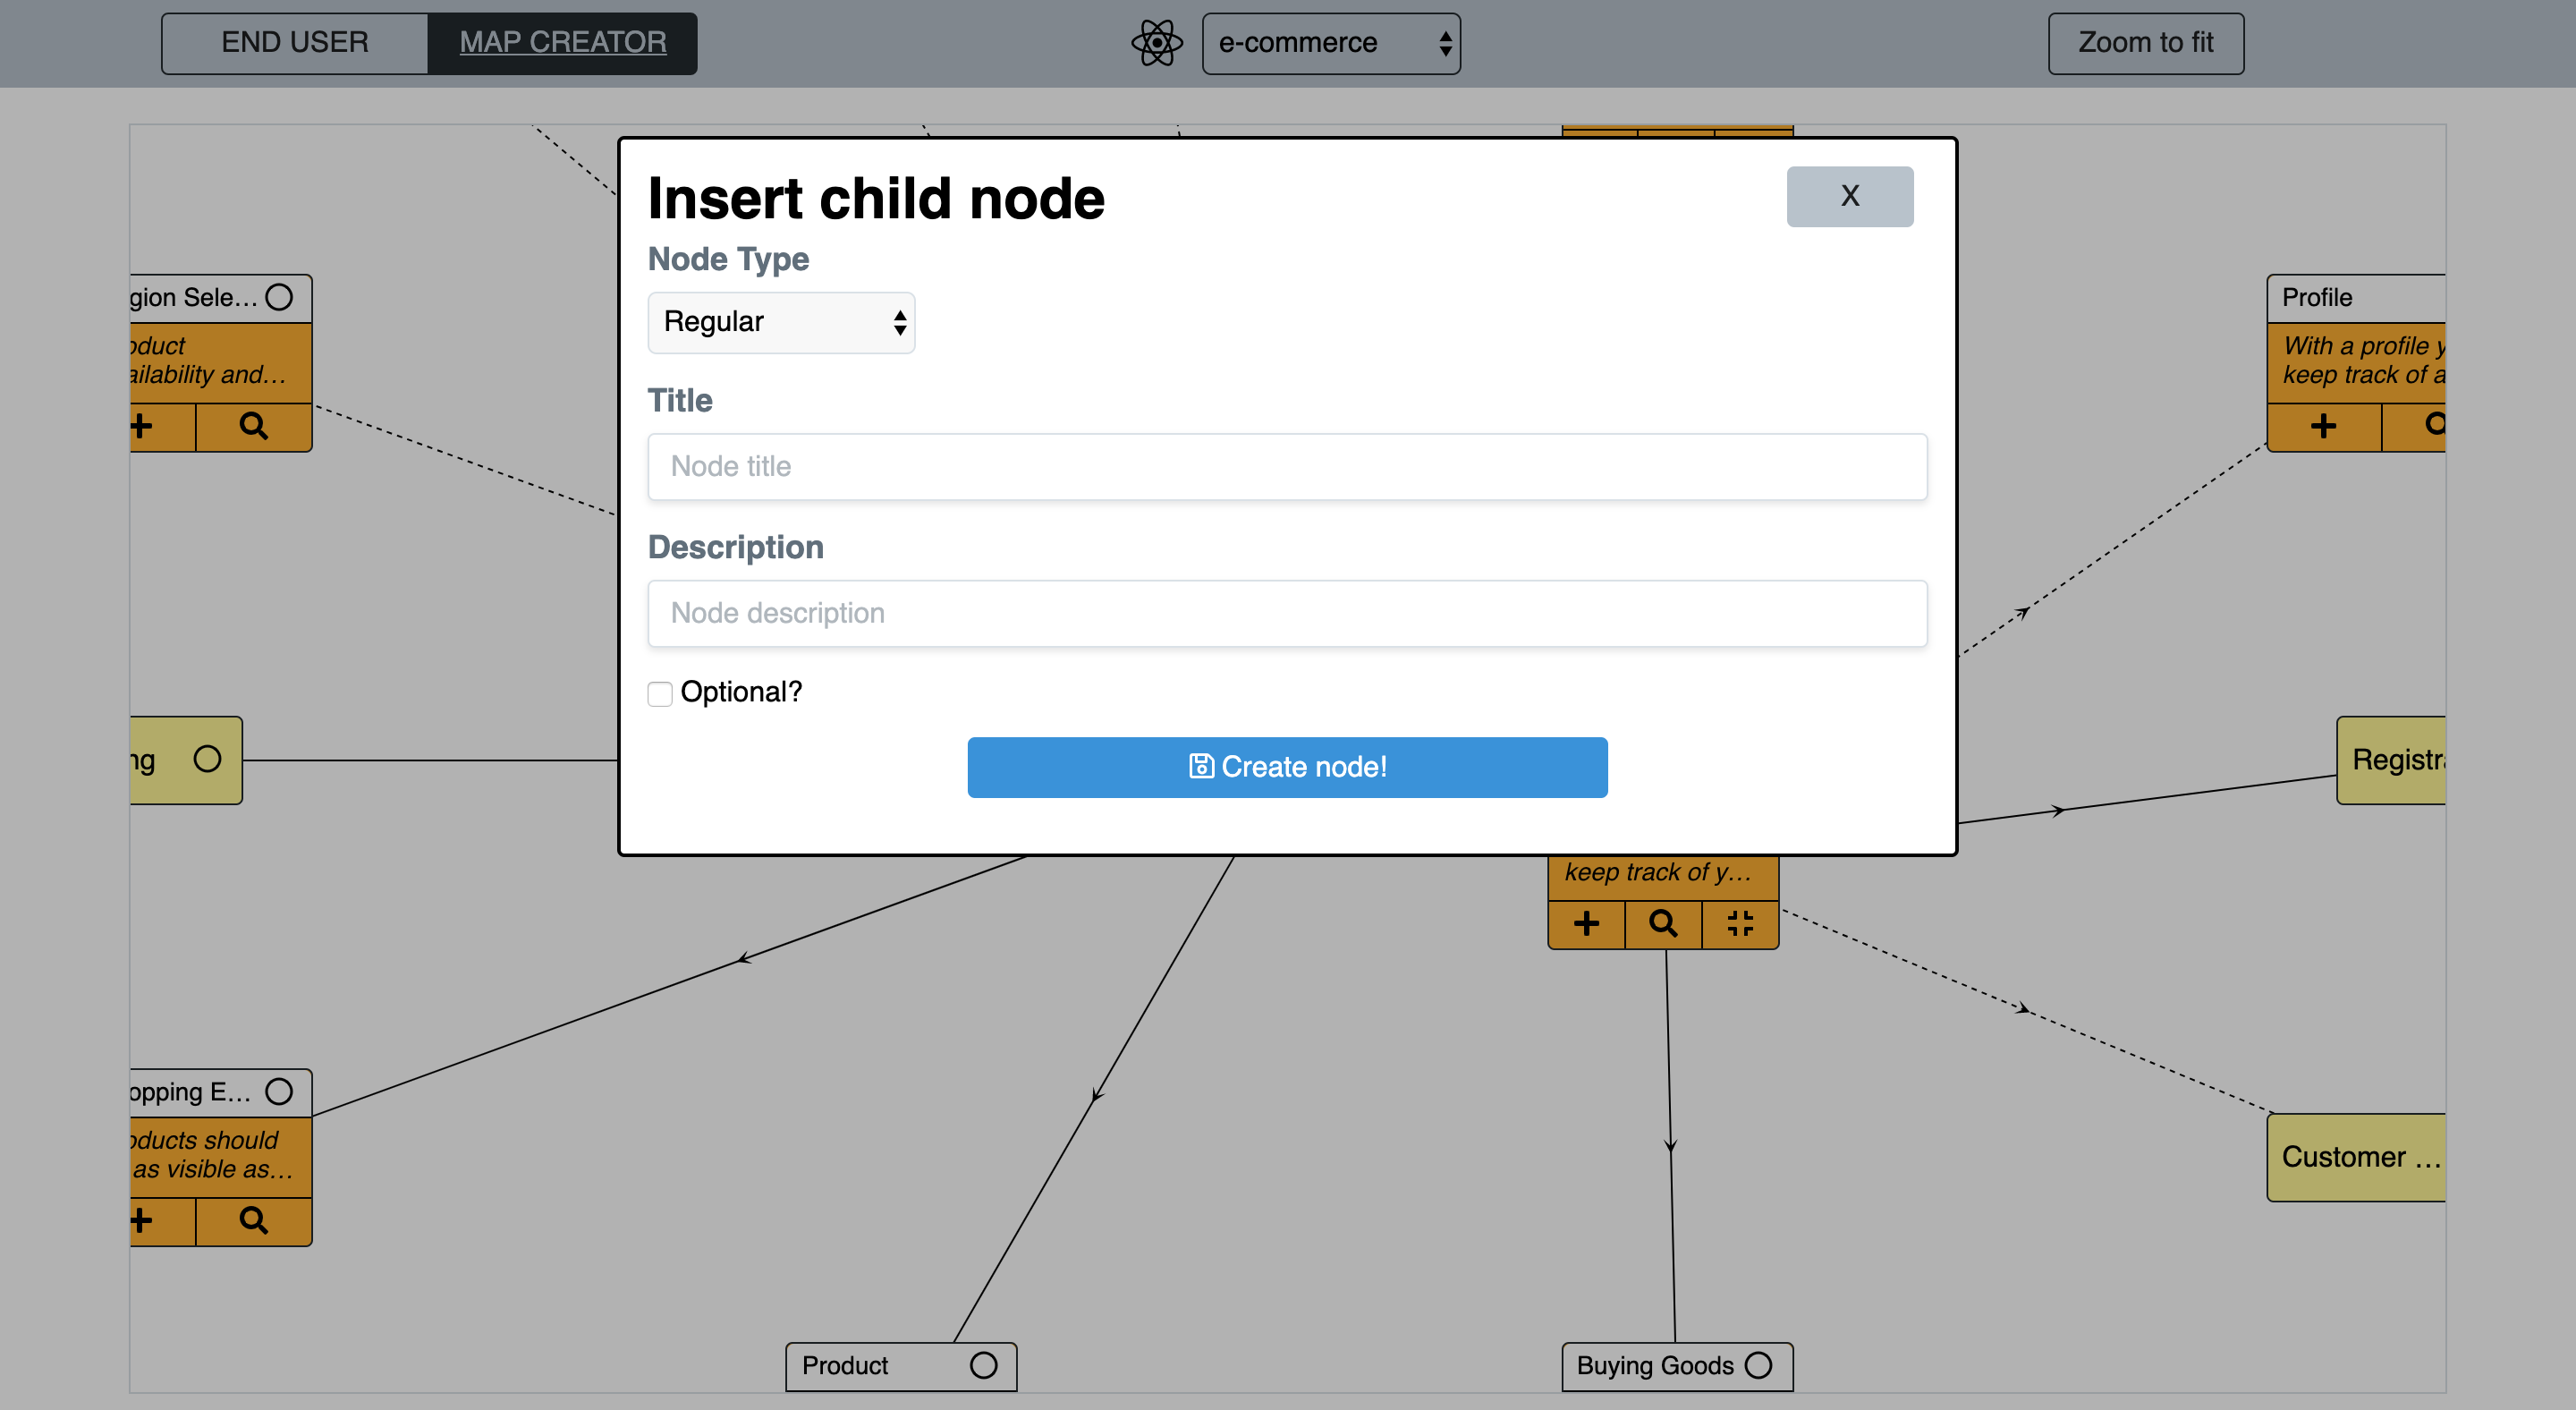
\includegraphics[width=\linewidth]{GMAddChildNodeModal-Regular.png}}
	\caption{Adding a regular node.}
	\label{fig:gm-add-regular}
\end{figure}



\subsubsection{EditModal Window}\label{sec:editmodal}
A click on the button to open the node opens a modal window containing the data. What this modal window looks like depends on the mode. If we are in map creator mode, a form will be shown to allow to change the title, the description, and the background color (see \autoref{fig:gm-editmodal-mapcreator}). In the case of the end-user mode (see \autoref{fig:gm-editmodal-enduser}), only the content and the background color can be changed. Only the first time a child node is added and no title and description is available yet, the end user is able to fill in these data as well.\\

When changing the background color, the user can choose to use the color also for all children or not. If the checkbox ``include children'' is checked, the background color of all child-nodes on all sublevels in the hierarchy will be changed to the new color. Otherwise, only the background color of the current node will be changed.\\

The text color is black by default. This can become a problem when the background color is changed to a dark color and certainly when it is black as well because then the text is not readable anymore. To solve this issue, we wrote some CSS rules that change the text-color depending on the background color. A black (or dark) background will result in white text and a white (or light) background results in black text.\\

The possibility to change the background color of the nodes and the fact that the text color is adapted taking the background color into account is also a useful feature for color-blind people. In this way, they can adapt the background colors of the nodes to colors they can distinguish better. Hence, requirement \ref{ur:accessibility} is achieved by this functionality.

\begin{figure}[H]
	\centering
	\frame{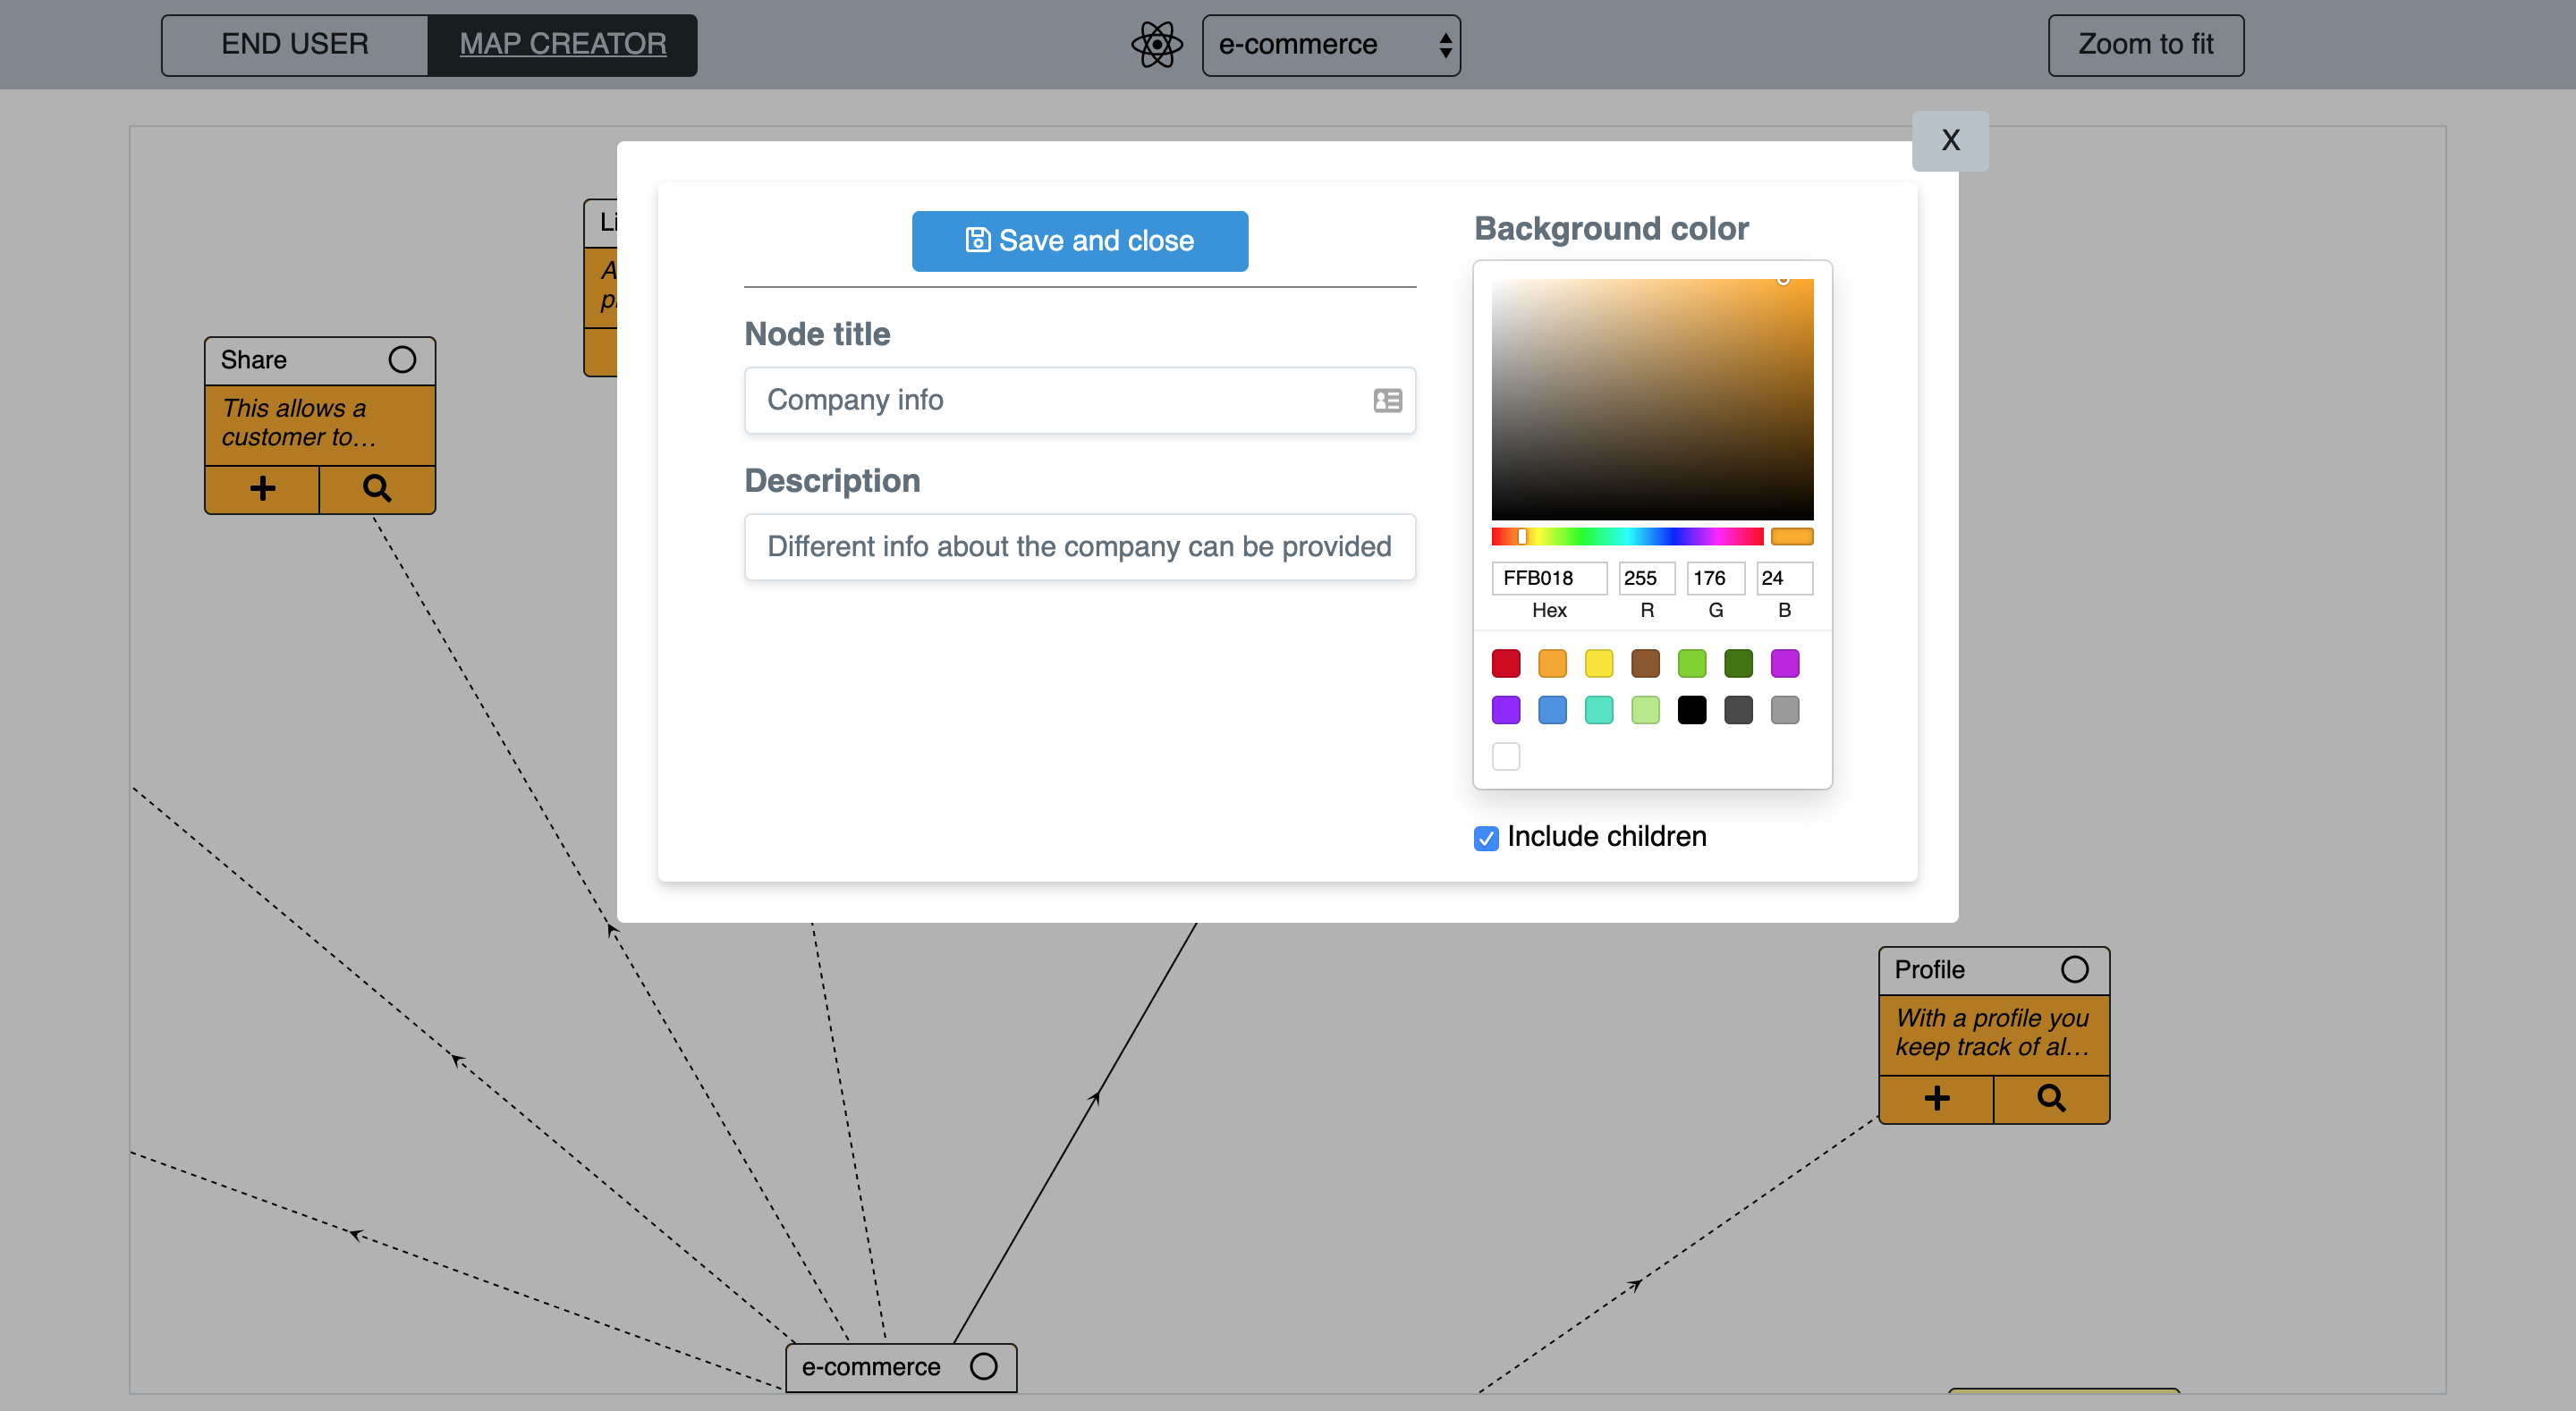
\includegraphics[width=\linewidth]{GMEditModal-MapCreator.png}}
	\caption{The edit modal in map creator mode.}
	\label{fig:gm-editmodal-mapcreator}
\end{figure}

\begin{figure}[H]
	\centering
	\frame{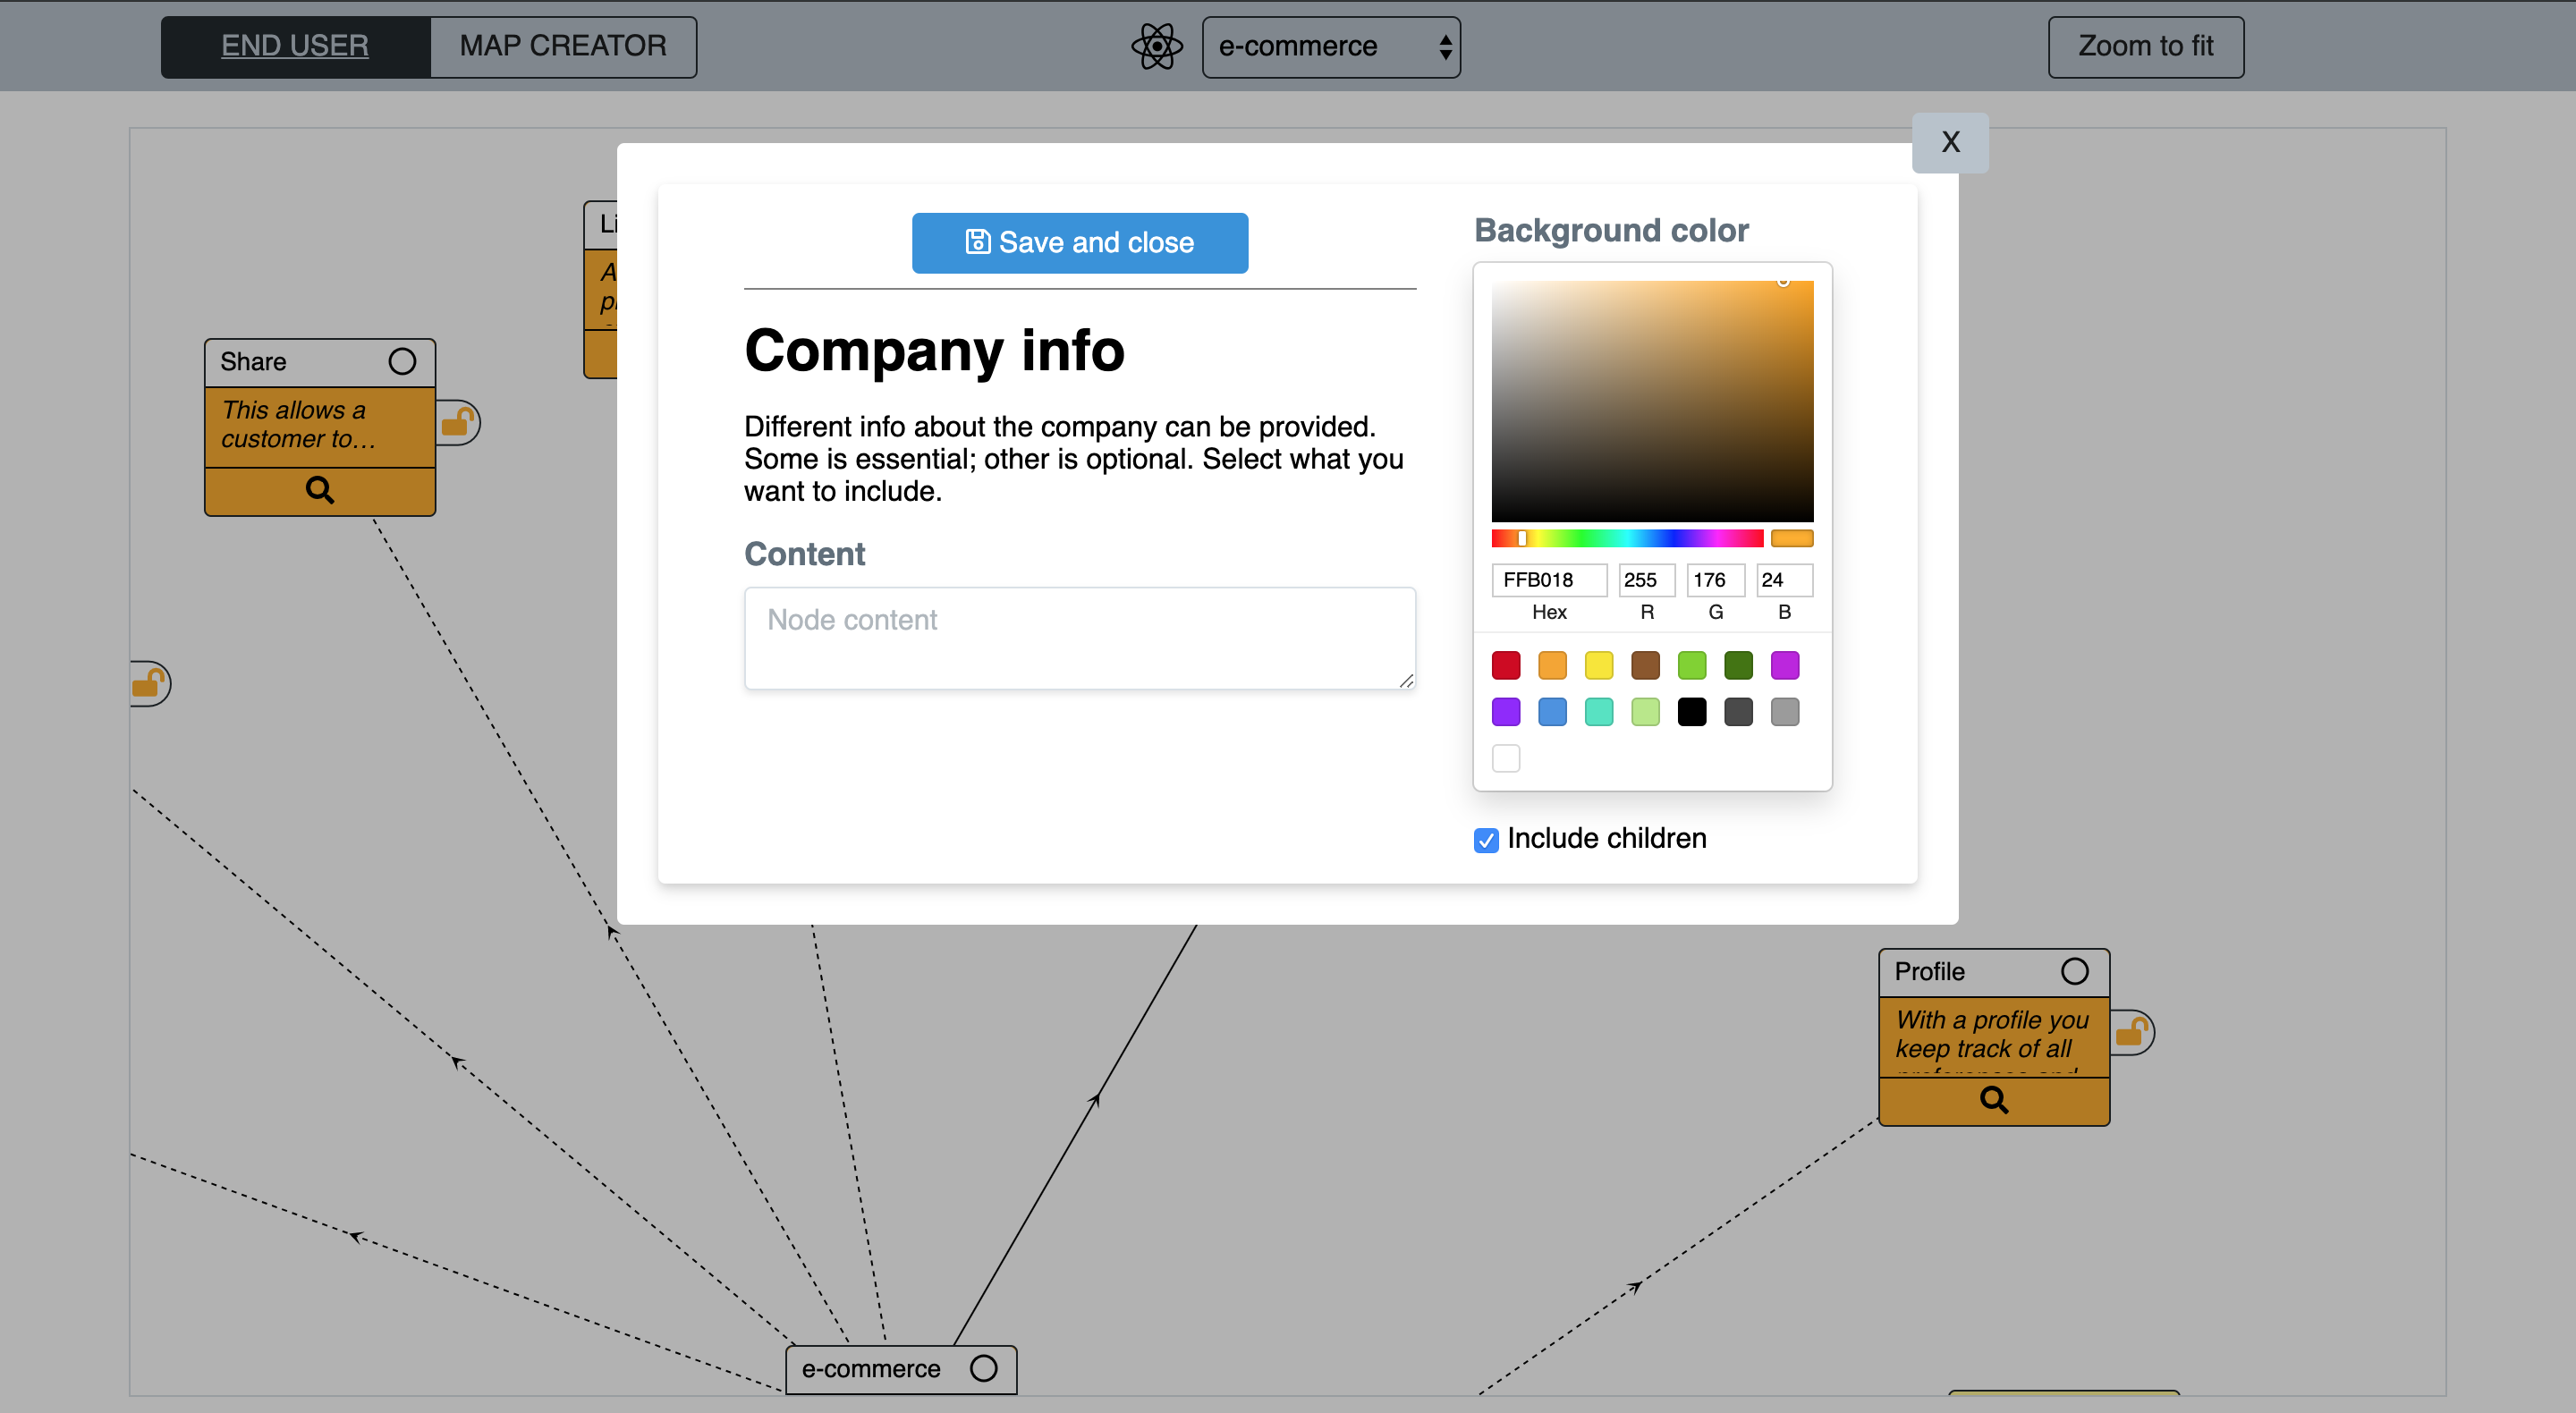
\includegraphics[width=\linewidth]{GMEditModal-EndUser.png}}
	\caption{The edit modal in end user mode.}
	\label{fig:gm-editmodal-enduser}
\end{figure}





% ----------------------------
% ------- CHOICE NODES -------
% ----------------------------
\subsection{Choice Nodes}
As explained in section \ref{sec:nodes}, choice nodes differ from the regular nodes in multiple ways. First the layout is different: while regular nodes have a title-, content- and controls-div, a choice node only has a title-div.\\

Remember that the purpose of a choice node is to let the user choose between different possibilities as children for the node. For example, the choice node with title ``Payment Method'' can have ``Cash'', ``Bancontact'' or other methods as child node. Depending on the situation, one (or more) of these methods can be chosen by the end-user.\\

It is the task of the map creator to define the possible choices the end-user can select. Therefore, when the map creator clicks on a button to add a child node, a similar modal window opens as shown in \autoref{fig:gm-add-choice}. The modal window provides text fields in which the map creator can insert a title and a description for the choice node, as well as the information for each choice, i.e. a title and a description. Because there is no maximum limit on the number of choices a map creator can provide, he can always ask to add more text fields to be able to give the information about an additional choice.\\

Another feature particular for choice nodes consists of the cardinalities a map creator can define. The map creator can set a lower limit and an upper limit. The lower limit is the minimum number of choices the end-user has to select. For example, if the lower limit is equal to two, the end-user cannot select only one choice. The upper limit is the maximum number of choices that can be selected by the end-user. By default the lower limit is equal to zero and the upper limit is equal to the total number of choices the map creator provided. It is not possible to set the upper limit equal to zero because this would not make sense: end-user would not be able to select any choice. Hence, the choice node would have no meaning and be useless.

\begin{figure}[H]
	\centering
	\frame{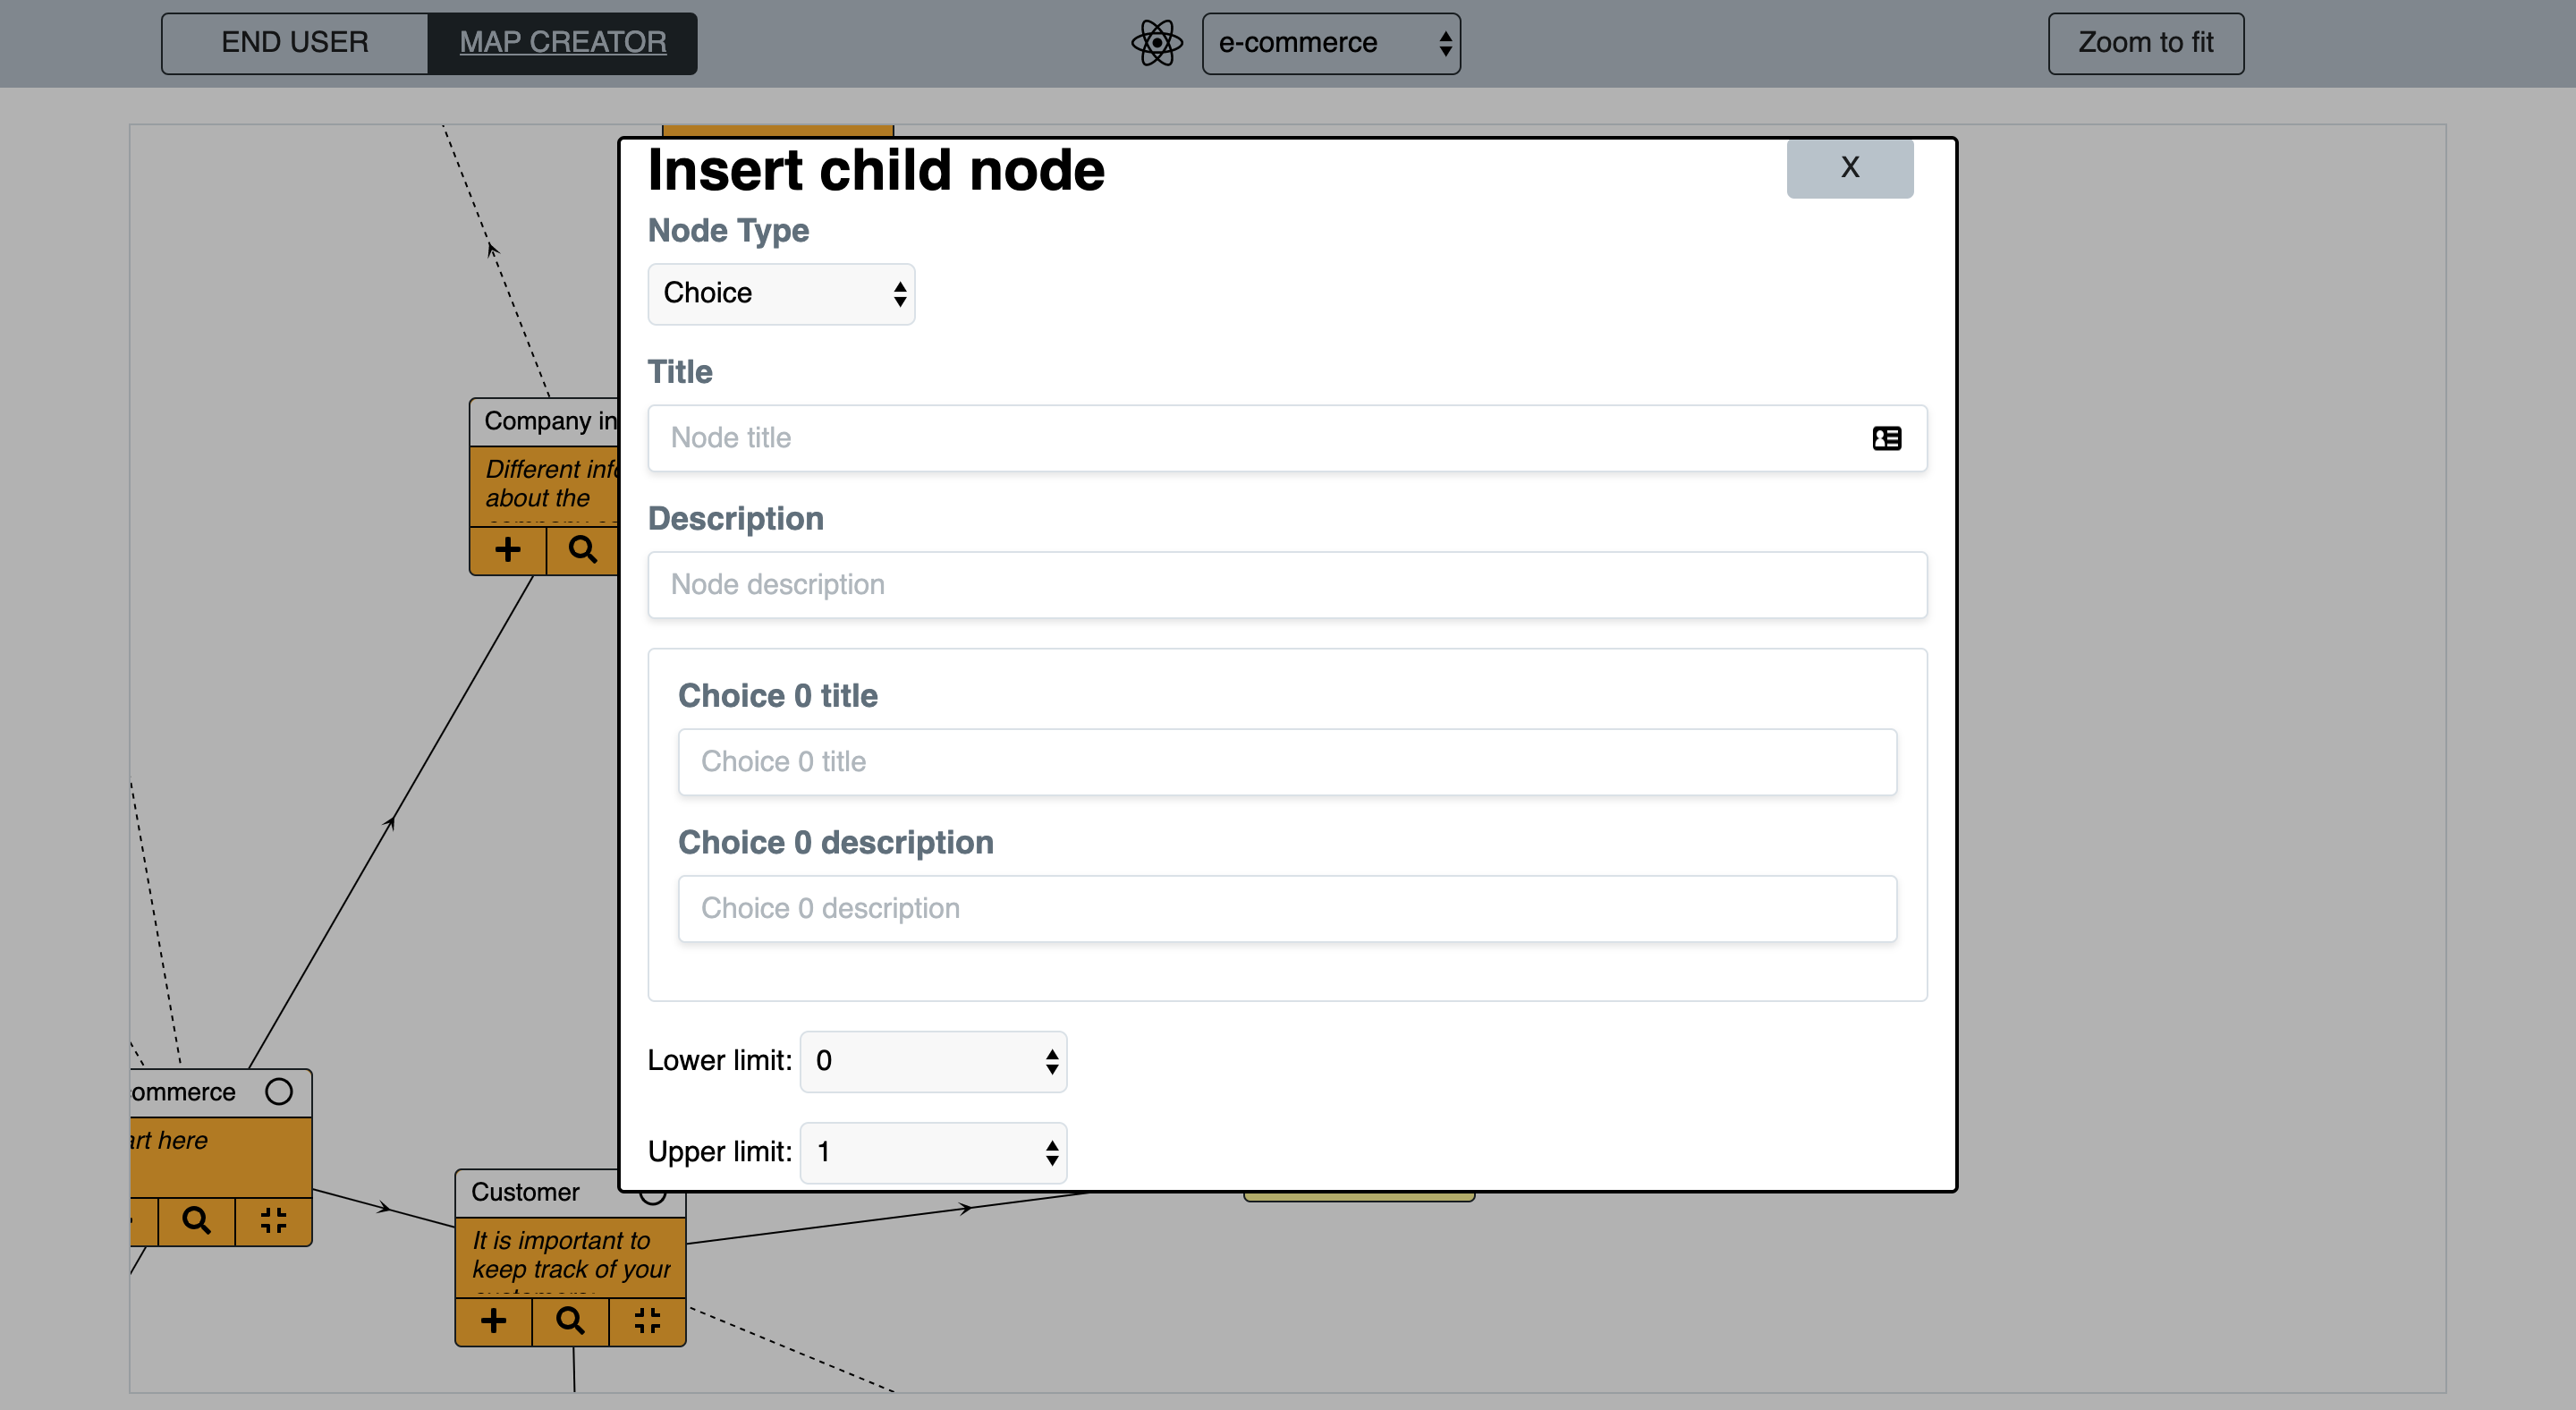
\includegraphics[width=\linewidth]{GMAddChildNodeModal-Choice.png}}
	\caption{Adding a choice node.}
	\label{fig:gm-add-choice}
\end{figure}

After the node is created, the map creator can edit the node by performing a single click on the choice node. Then a modal window opens and he can edit the title, the description and the already defined choices (see \autoref{fig:gm-choicenode-mapcreator}). To delete a choice, the map creator only has to empty the text fields of the choice.

\begin{figure}[H]
	\centering
	\frame{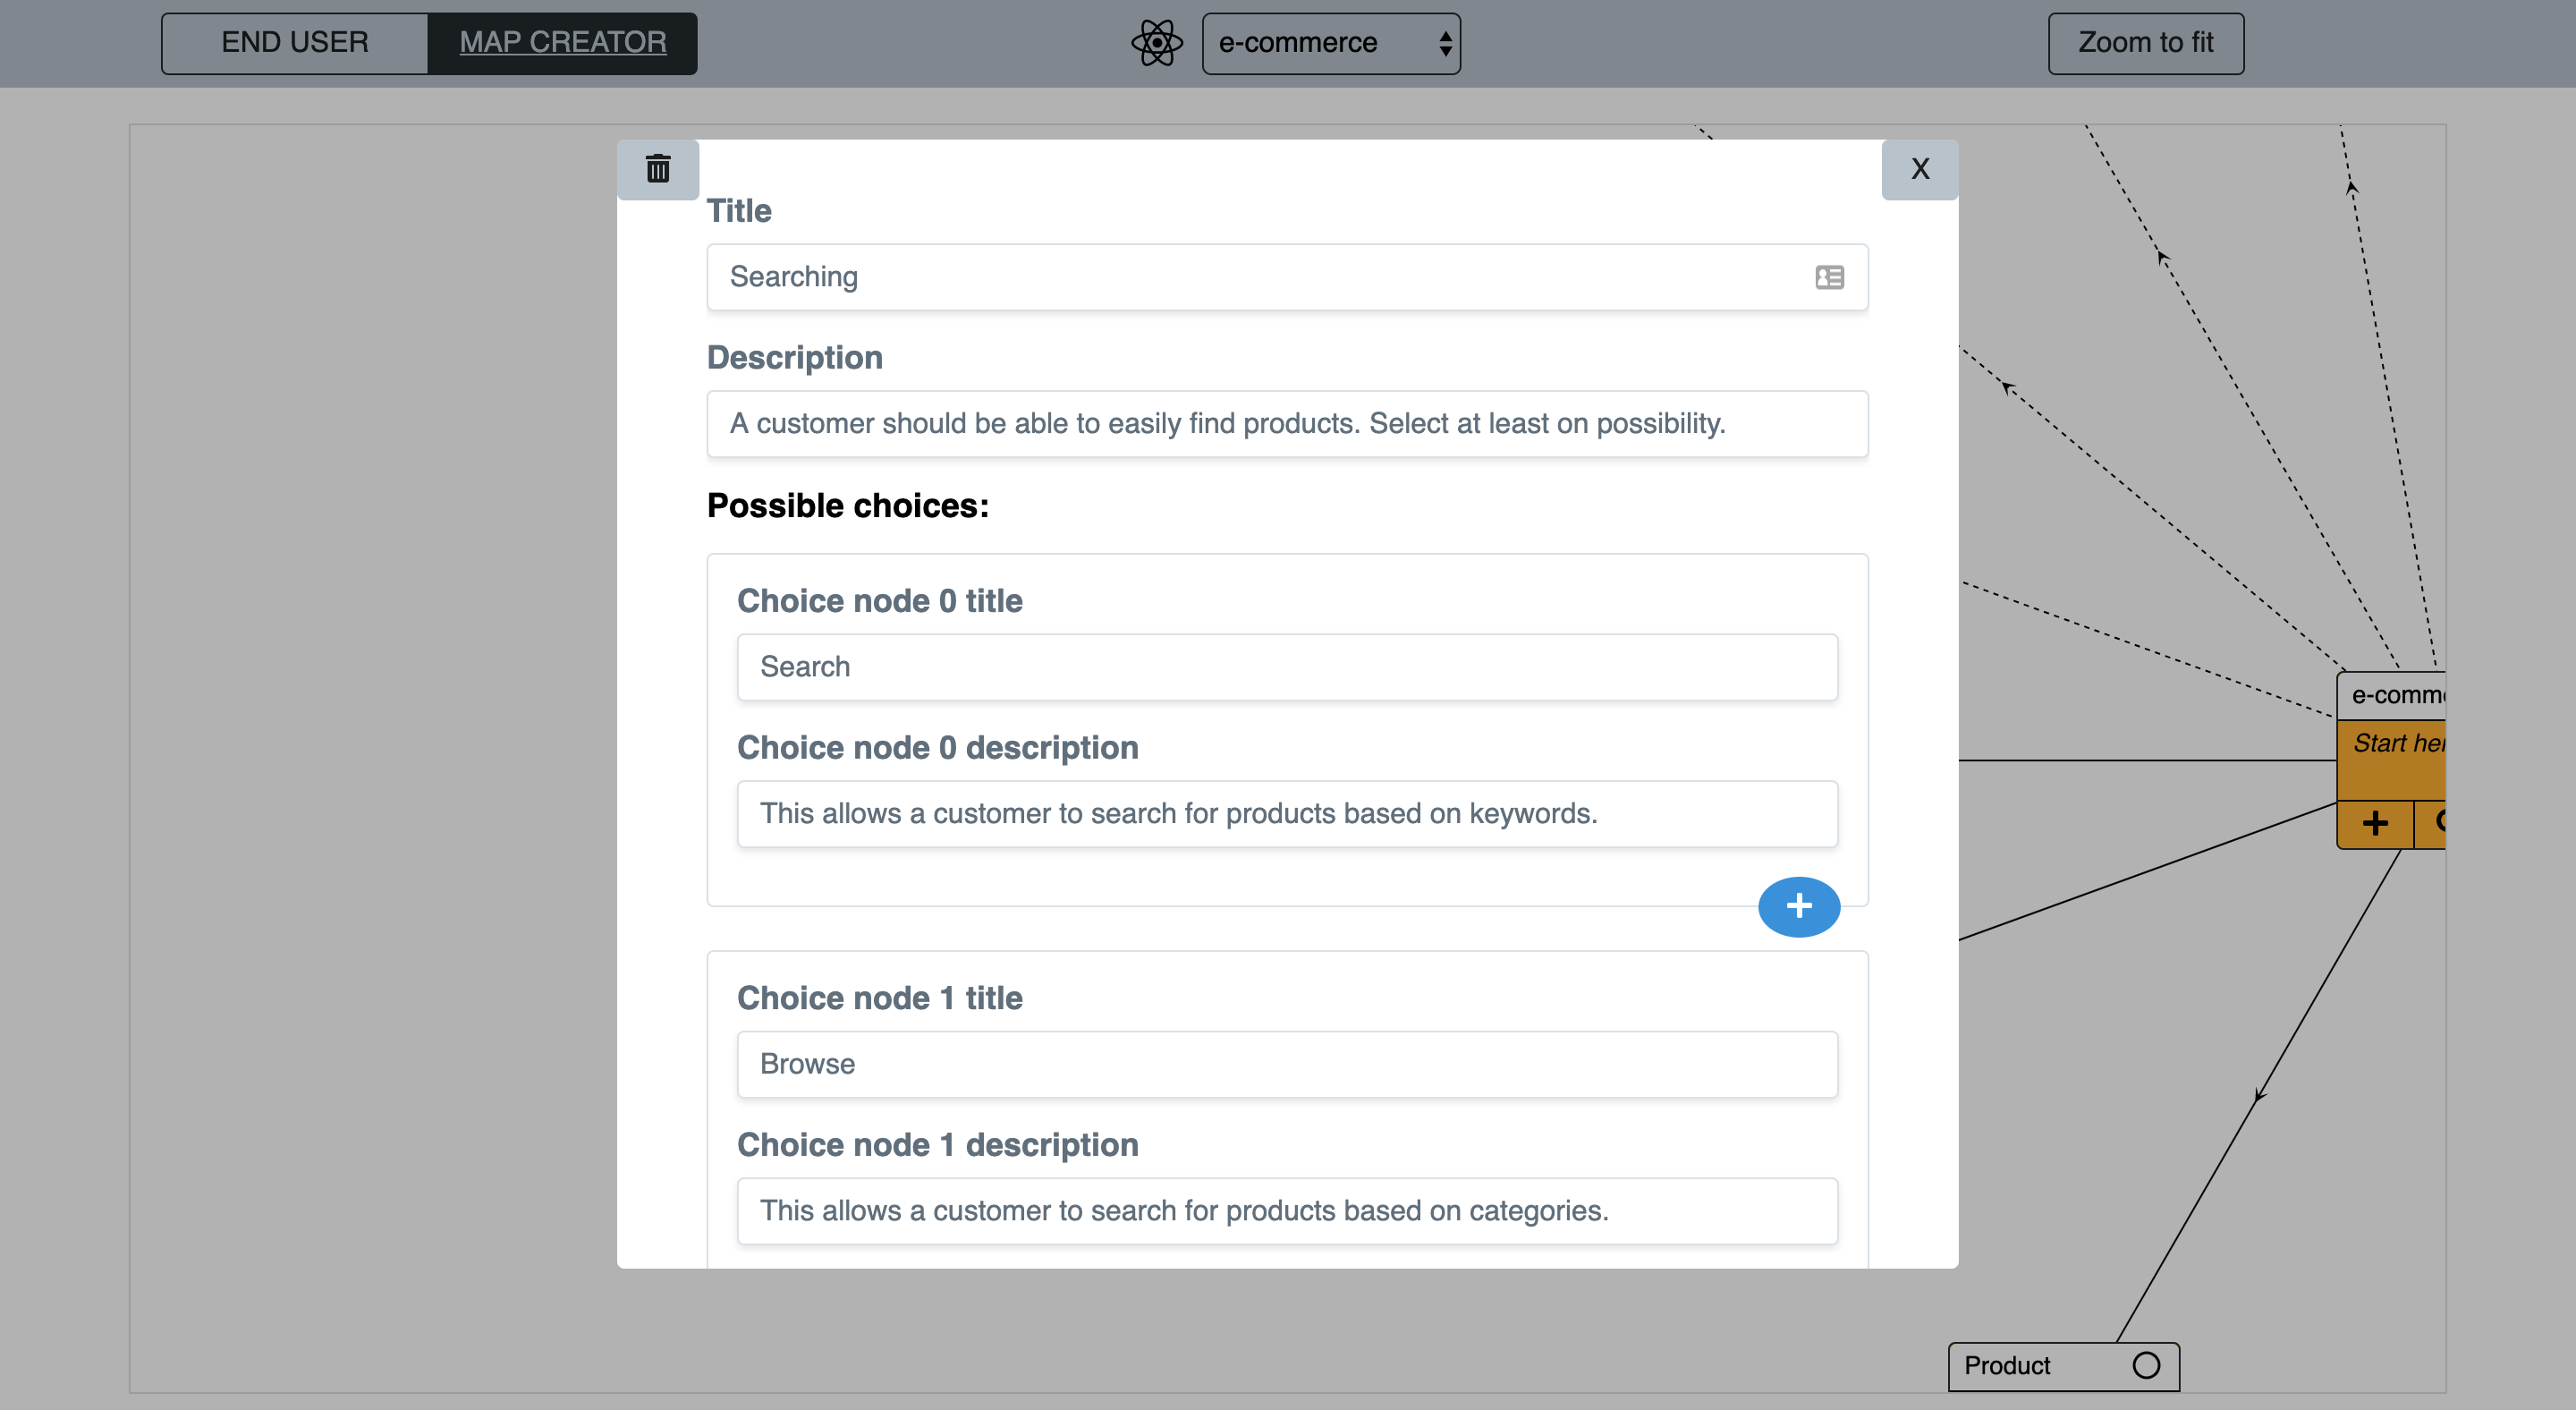
\includegraphics[width=\linewidth]{GMChoiceNode-MapCreator.png}}
	\caption{An opened choice node in map creator mode.}
	\label{fig:gm-choicenode-mapcreator}
\end{figure}

The modal window showing up when the end-user clicks on a choice node (see \autoref{fig:gm-choicenode-enduser}) is not equal to the modal window the map creator can see after the same action. The end-user sees the title and description of the node on top, but (s)he cannot edit these like a map creator. Under the description is shown how many choices the end-user should select. For example ``Select between 1 and 3 choices'', where 1 is the lower limit and 3 the upper limit set by the map creator. This instruction is followed by a form, where every possible choice is made visible by showing the title and the description. The end-user can select the choices he wants via a checkbox. With a click on the button, the selected choices are registered and added as children to the choice node. It is possible at any time to adapt the choices by reopening the modal window. At that moment, the checkbox(es) of the previously selected choice(s) will be checked. To remove a choice as child of the choice node, it is sufficient to uncheck the checkbox.\\

Next to selecting choices given by the map creator, it can sometimes be necessary to be able to add an extra possibility, which was not given by the map creator. Therefore, an end-user can create additional choices, which he can select later on. Additional choices can be created in the same way as the map creator can do it. By a click on the button, an additional part of the form appears in the modal window. When the form is submitted, the additional choice is registered with the given title and description. An example is shown in \autoref{fig:gm-choicenode-enduser-extraoption}.
\begin{figure}[H]
	\centering
	\frame{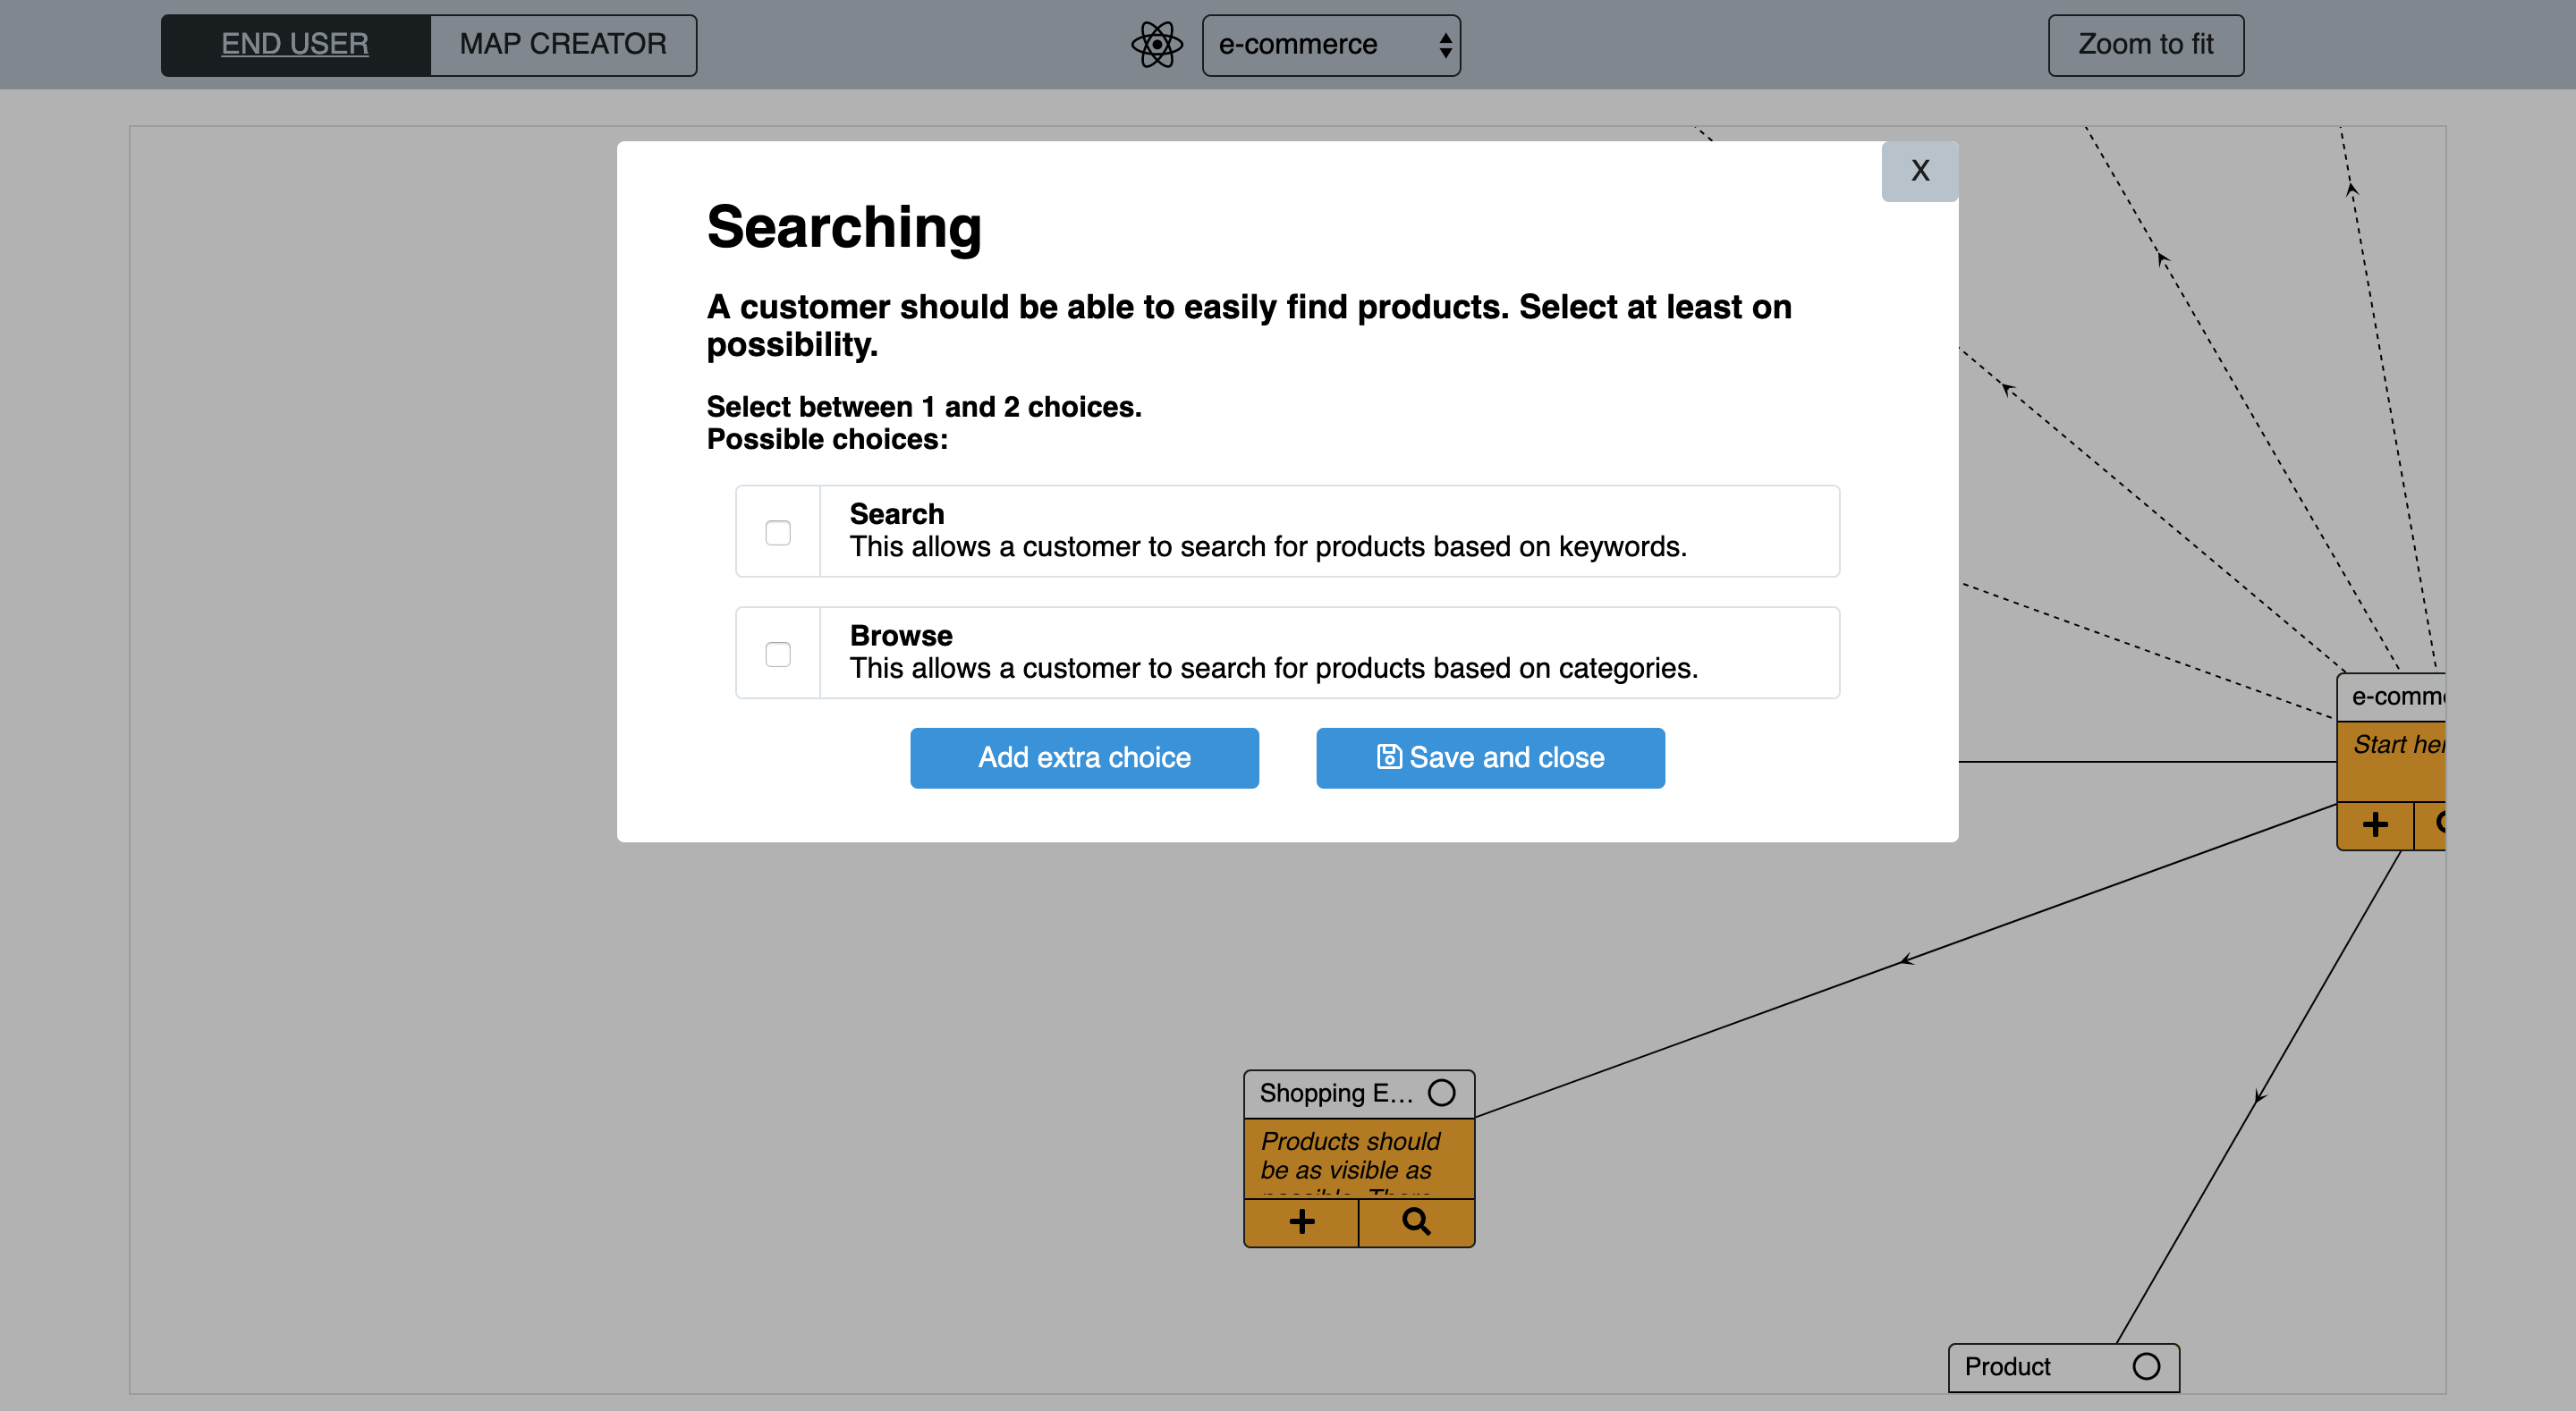
\includegraphics[width=\linewidth]{GMChoiceNode-EndUser.png}}
	\caption{An opened choice node in end user mode.}
	\label{fig:gm-choicenode-enduser}
\end{figure}

\begin{figure}[H]
	\centering
	\frame{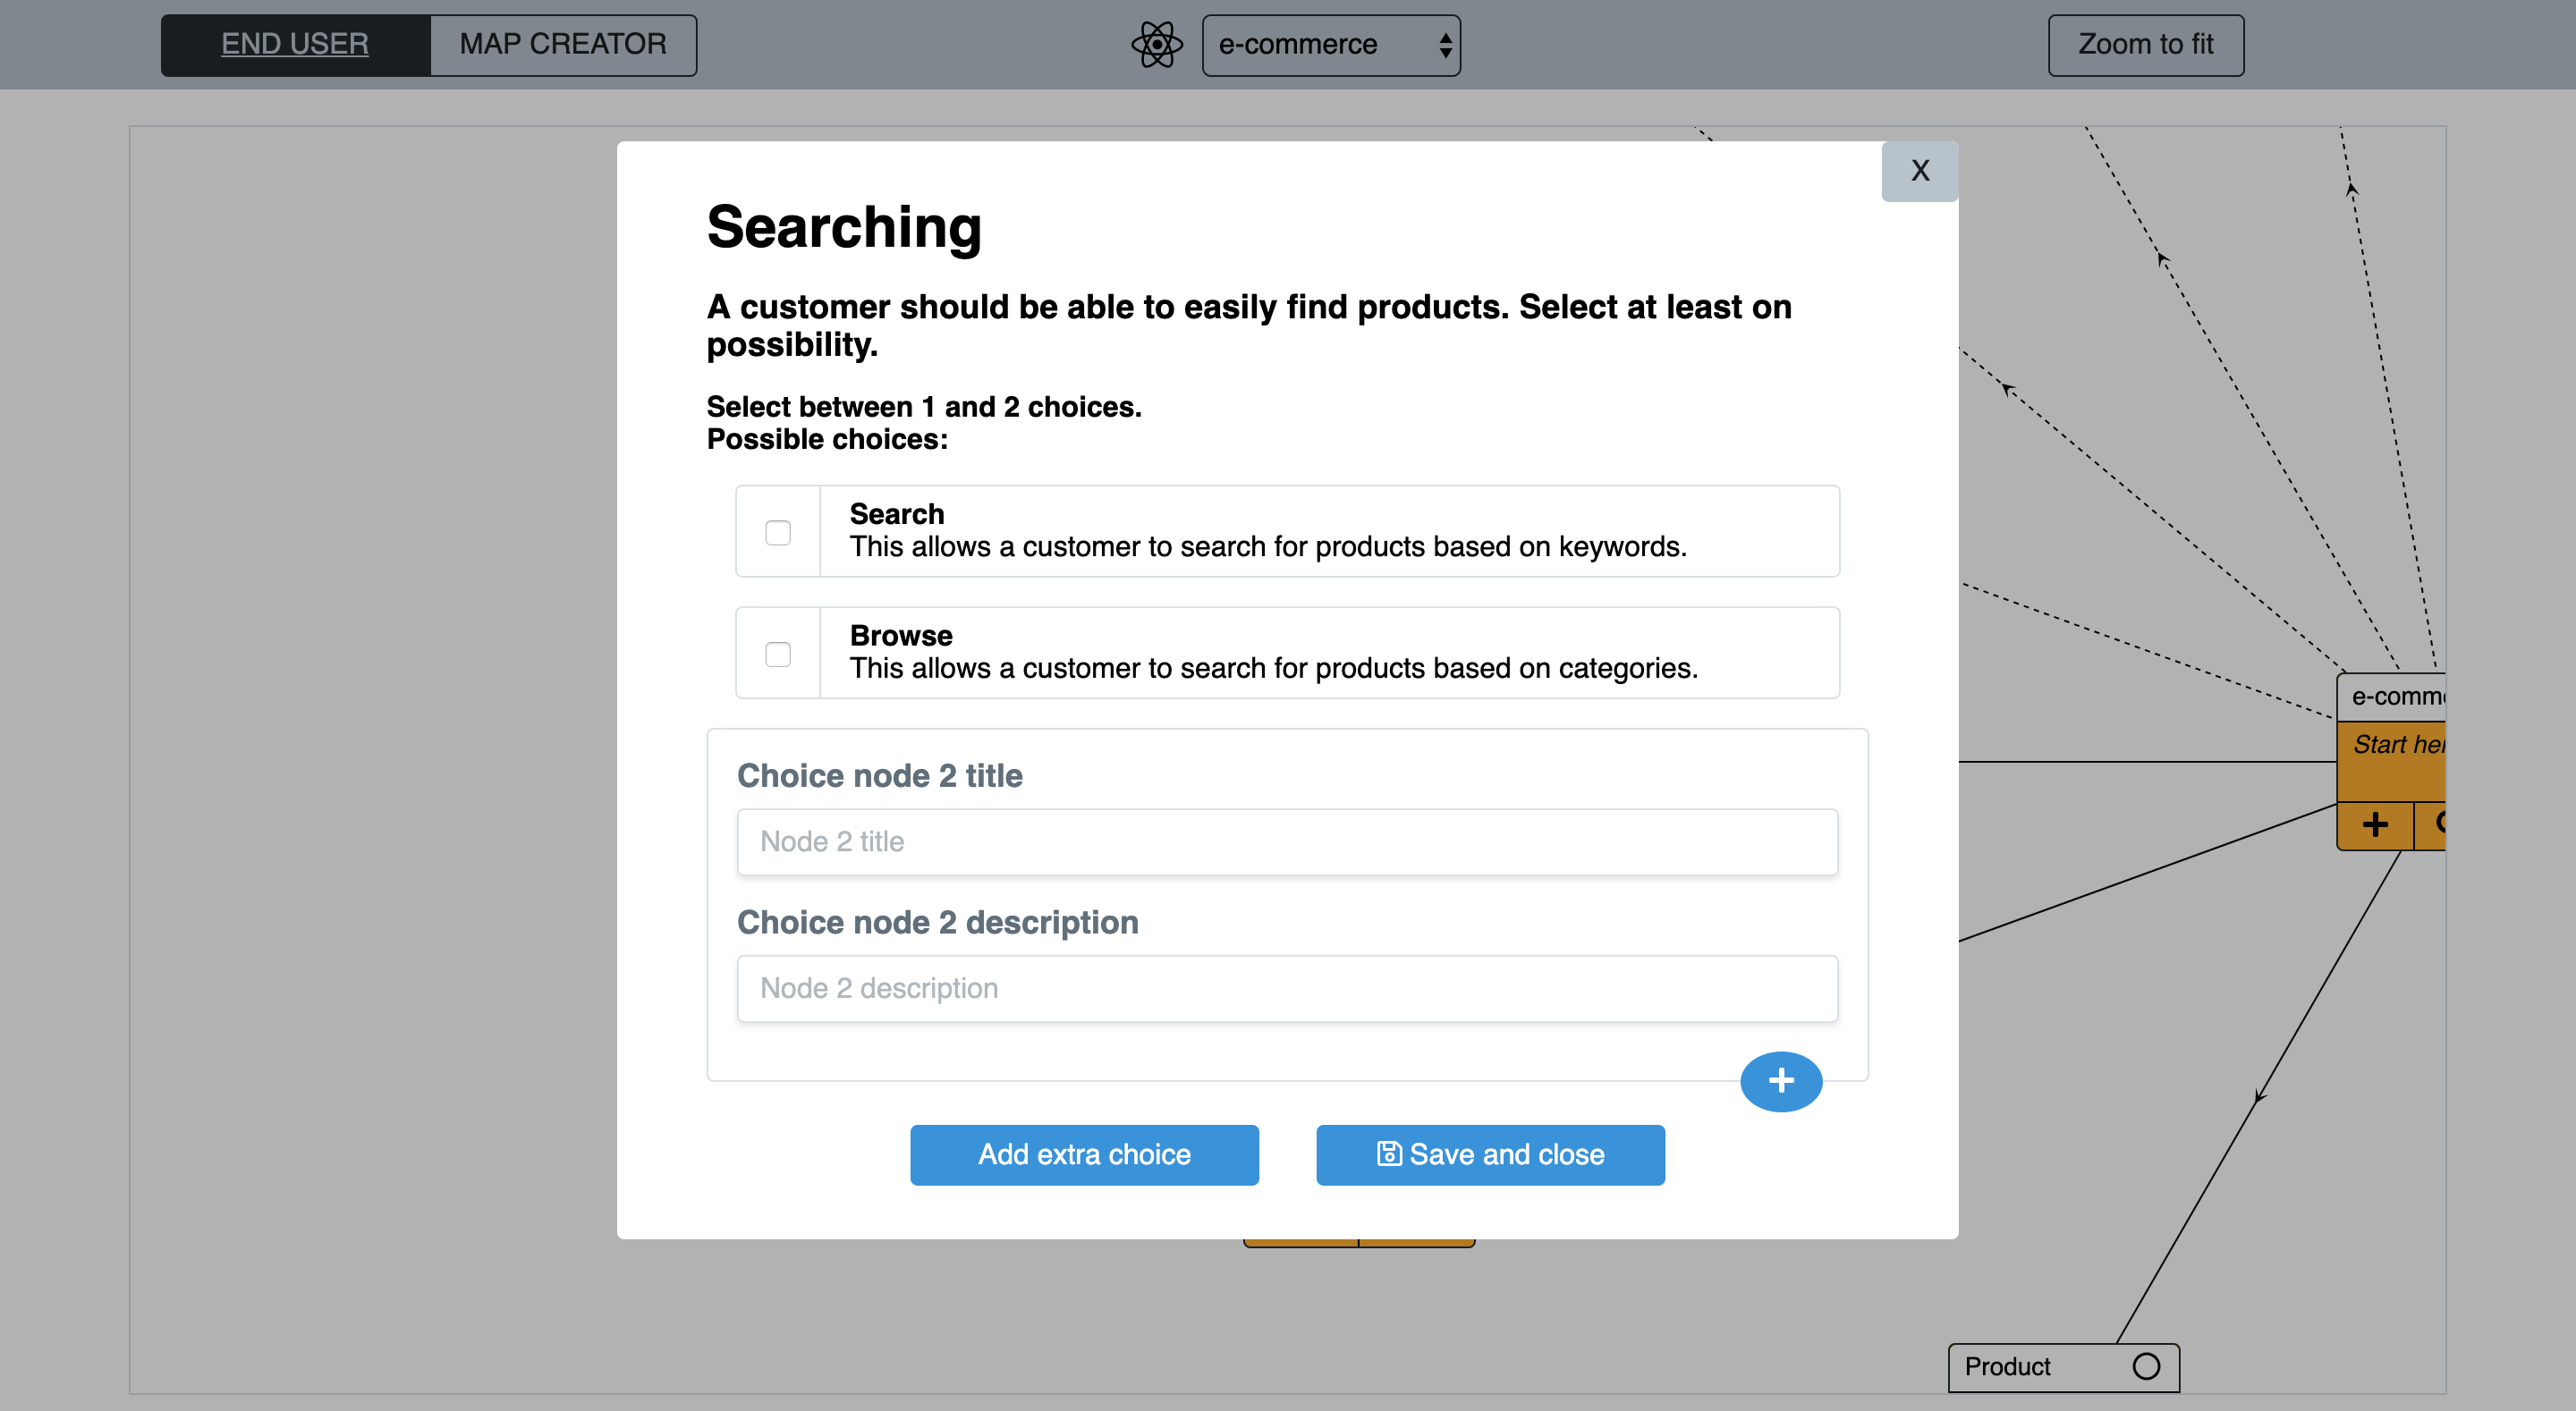
\includegraphics[width=\linewidth]{GMChoiceNode-EndUser-ExtraOption.png}}
	\caption{An opened choice node in end user mode with option to select additional choice.}
	\label{fig:gm-choicenode-enduser-extraoption}
\end{figure}



% ----------------------------
% ------ OPTIONAL NODES ------
% ----------------------------
\subsection{Optional nodes}\label{sec:optional-nodes}
A map can also provide optional nodes. They can be recognized by the dotted link between this node and its parent. A special characteristic of optional nodes is that these nodes can be disabled by the end-user. Therefore, optional nodes contain an additional button, represented as a lock, at their right side. As long as the node is enabled, the button is represented by an open lock. A click on this button disables the node and changes the icon into a closed lock. The node can be enabled again by clicking the lock again. Next to the lock icon, a disabled node can be recognized by its gray background and a blurred content so that the content is less readable.\\

A second characteristic of optional nodes is that they do not contribute to the ``completeness icon'' of the visualization. Hence, to determine whether the completeness icon of a node should be empty, filled or partially filled, optional child nodes and their descendants (which are optional as well) are skipped because it does not matter whether content is provided in these nodes or not. There is only one exception on this rule: when a choice node is optional but it does have children (selected by the end-user), these children are not optional and are checked for completeness.














